% Generate PDF version 1.7 (needed for proper integration of .eps)
% Prevents this warning: "PDF inclusion: found PDF version <1.7> [...]"
\pdfminorversion=7

\RequirePackage{amsmath}
\documentclass[runningheads]{llncs}
%\documentclass[runningheads,12pt]{llncs}

%\usepackage[letterpaper, margin=1in]{geometry}

%%%%%%%%%%
% HEADER %
%%%%%%%%%%

\usepackage{algorithm}
\usepackage[noend]{algpseudocode}  % layout for algorithmicx

% commonly used packages, commands, etc.
%%%%%%%%%%%%%%%%%%%
%    PACKAGES     %
%%%%%%%%%%%%%%%%%%%

\usepackage[utf8]{inputenc} % enable UTF-8
\usepackage{lipsum} % write pseudo text

% images
\usepackage{graphicx}

% Why `\usepackage[T1]{fontenc}'?
% https://tex.stackexchange.com/questions/664/why-should-i-use-usepackaget1fontenc
% If you don't use \usepackage[T1]{fontenc},
% - Words containing accented characters cannot be automatically hyphenated,
% - You cannot properly copy-and-paste such words from the output (DVI/PS/PDF),
% - Characters like the pipe sign, less than and greater sign give unexpected
%   results in text.
\usepackage[T1]{fontenc}


%%%%%%%%%%%%%%%%%%%
% REQUIRED INPUTS %
%%%%%%%%%%%%%%%%%%%

% mark overfull boxes
% Description: This file enables marking overfull boxes, \eg, words that extend
% beyond the end of the line
%
% Usage: Create file headers/config/showoverfull.config

\IfFileExists{headers/config/showoverfull.config}{
	%\usepackage{showframe}
	\overfullrule=1cm
}{
	% no action necessary
}

% comments
% Description: This file defines commands for comments
%
% Usage: % Description: This file defines commands for comments
%
% Usage: \input{headers/lqa/comments}
%
% Requires packages (already included in template):
% - \usepackage[usenames, dvipsnames]{color}

% TODO markers
% the optional argument indicates the person who created the TODO
\newcommand{\todo}[2][]{
	\write16{^^JTODO on page \thepage: #2^^J}
	\textcolor{red}{\textbf{TODO #1:} #2}
}

%% >>> BEGIN NO PARSE
\newenvironment{commentlist}{
\color{gray}
\begin{itemize}
}
{
\end{itemize}
}
%% >>> END NO PARSE

%
% Requires packages (already included in template):
% - \usepackage[usenames, dvipsnames]{color}

% TODO markers
% the optional argument indicates the person who created the TODO
\newcommand{\todo}[2][]{
	\write16{^^JTODO on page \thepage: #2^^J}
	\textcolor{red}{\textbf{TODO #1:} #2}
}

%% >>> BEGIN NO PARSE
\newenvironment{commentlist}{
\color{gray}
\begin{itemize}
}
{
\end{itemize}
}
%% >>> END NO PARSE


% appendix
\clearpage
\appendix

\section{Appendix} \label{sec:appendix}
\subsection{Generic Algorithms: \A and \dijkstra} \label{TRIEapp:astar}

\cref{TRIEalg:generic-alignment} shows a generic implementation of the \A algorithm,
roughly following~\cite{dechter_generalized_1985}.
We do not implement the reconstruction of the best alignment in order to simplify the presentation.
The procedure \mbox{\textsc{BacktrackPath}} traces the best alignment back to the $source$, based on remembered edges used to optimize $f$ for each alignment state.
%
\cref{TRIEalg:generic-alignment} also shows a simple implementation of Dijkstra in
terms of \A.

\begin{algorithm}[H]
	\caption{\A algorithm (generalizes Dijkstra)}\label{TRIEalg:generic-alignment}
	\begin{algorithmic}[1]
				
		\Function{\A}{$G\colon \text{Graph}$,
			$S\colon \text{Sources}$,
			$T\colon \text{Targets}$,
			$h\colon \text{Heuristic function}$}
		\State $f \gets \mli{Map}(\mli{default}=\infty)\colon
		\text{Nodes} \to \mathbb{R}_{\geq 0}$
		\Comment Map nodes from $G$ to priorities 
		\State $Q \gets \mli{MinPriorityQueue}(\mli{priority}=f)$ 
		\Comment Priorities according to $f$
		\ForAll{$s \in S$}
			\State $f[s] \gets 0.0$
			\State $Q.\mli{push}(s)$
			\Comment Initially, explore all $s \in S$
		\EndFor
		\While{$Q \neq \emptyset$}
			\State $\mli{curr} \gets Q.\mli{pop}()$
			\Comment Get state with minimal $f$ to be expanded
			\If{$\mli{curr} \in T$}
				\State \Return \Call{BacktrackPath}{$\mli{curr}$}
				\Comment Reconstruct a path to $\mli{curr}$ (omitted)
			\EndIf
				\ForAll{$(\mli{curr},\mli{next},\mli{cost}) \in
				G.\mli{outgoingEdges}(\mli{curr})$}
			\State $\hat{f}_\mli{next} \gets f[\mli{curr}] + \mli{cost} +
			h(\mli{next})$
				\Comment Candidate value for $f[\mli{next}]$
				\If{$\hat{f}_\mli{next} < f[\mli{next}{}]$}
					\State $f[\mli{next}] \gets \hat{f}_\mli{next}$		
					\State $Q.\mli{push}(\mli{next})$
					\Comment Explore state $\mli{next}$
				\EndIf
		\EndFor
		\EndWhile
		\State \textbf{assert} $\mli{False}$
		\Comment Cannot happen if $T$ is reachable from $S$
		\EndFunction

		\Statex

		\Function{Dijkstra}{$G\colon \mli{Graph}$,
			$S\colon \mli{Sources}$,
			$T\colon \mli{Targets}$}
			\State $h(v) \gets 0.0$
			\Comment Constant-zero function $h$
			\State $\Call{\A}{G,S,T,h}$
		\EndFunction
	\end{algorithmic}
\end{algorithm}
           %% HIGHER PRIORITY
\newpage
\subsection{Recursive Alignment Algorithm} \label{app:recursive-align}
\cref{alg:recursiveAlign} shows our implementation of \textsc{RecursiveAlign},
used in \cref{TRIEalg:astarix} to evaluate $h$. \textsc{RecursiveAlign} is a simple
branch-and-bound algorithm that recursively looks for the cheapest alignment of
$s$ starting from $u$, and does not follow paths whose cost exceeds
$\mli{best}$, the best path found so far.

\begin{algorithm}[t]
	\caption{Recursive alignment used by Heuristic in \cref{TRIEalg:astarix}.}\label{alg:recursiveAlign}
	\begin{algorithmic}[1]
		\Statex
			\Function{RecursiveAlign}{$u, s, \mli{curr}, \mli{best}$} \Comment
			Return value is $\leq \mli{best}$
			\If{$\mli{curr} \geq \mli{best}$}
				\State \Return $\mli{best}$
				\Comment Branch and bound: bounding
			\EndIf
			\If{$s = \epsilon$}  % \textbf{or} $u = \mli{border}$}
				\Comment Reached a target
				\State \Return $\mli{curr}$
			\EndIf
			\ForAll{$(u,\mli{v},\ell,w) \in
				\AGE \textbf{ where } \ell \in \{s[0], \epsilon \}$}
				\State $\mli{suff} = s[1:]$ \textbf{if} $\ell \neq \epsilon$ \textbf{else} $s$
				\State $\mli{best} = \Call{RecursiveAlign}{u, \mli{suff}, curr + w, \mli{best}}$
			\EndFor
			\State \Return $\mli{best}$
		\EndFunction
	\end{algorithmic}
\end{algorithm}
       %% HIGHER PRIORITY
%\newpage
\subsection{Parameter Estimation} \label{subsec:parameter_estimation}
We now evaluate the influence of different parameter choices ($\costcap$, $d$,
$D$) on runtime and memory usage.

\begin{figure}[H]
	\centering
	\begin{minipage}{0.48\linewidth}
		\centering
		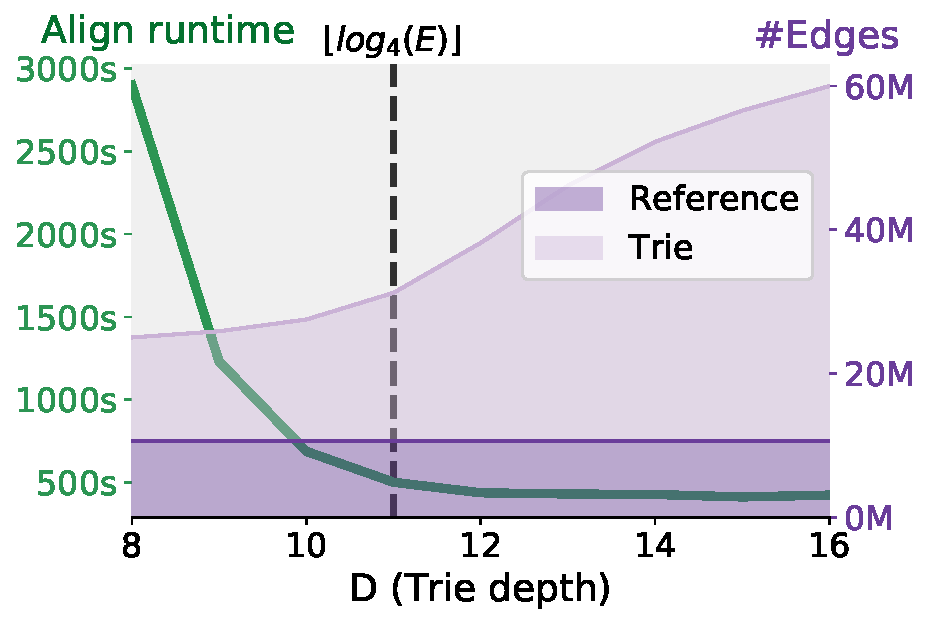
\includegraphics[width=\linewidth]{figs/trie/MHC1-trie-vs-D.pdf}
		\caption[Effect of $D$ on performance of \astarix]{Effect of $D$ on performance of \astarix (MHC1 experiment). The dashed line shows our choice of $D$.}
		%\label{subfig:MHC1-trie_vs_D}
		\label{fig:trie_vs_D}
	\end{minipage}~\hspace{0.7em}
	\begin{minipage}{0.49\linewidth}
		\centering
		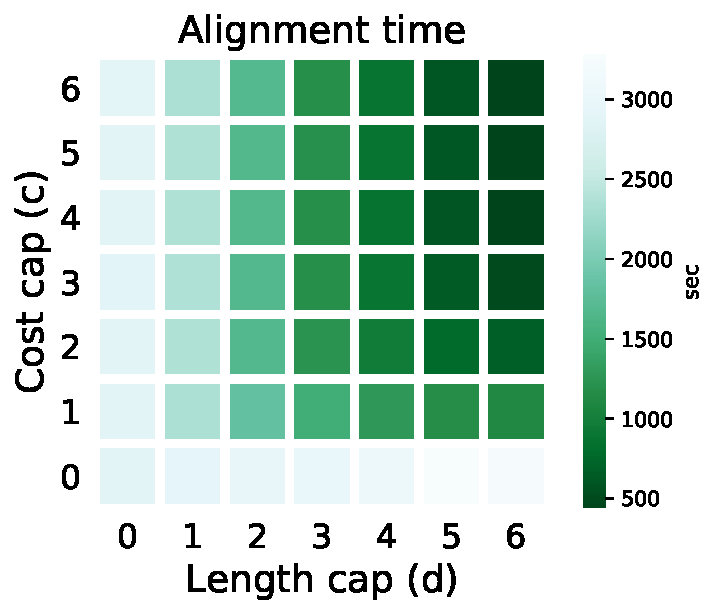
\includegraphics[width=0.8\linewidth]{figs/heuristic/MHC1-heatmap-c_vs_d-align_sec.pdf}
		\caption[Runtime of \astarix depending on $d$ and $\costcap$]{Runtime of \astarix depending on $d$ and $\costcap$ (MHC1 experiment).}
		\label{fig:heuristic-parameters}
	\end{minipage}
\end{figure}

\cref{fig:trie_vs_D} demonstrates the benefit of using a trie with the size
reduction optimization (end of \cref{subsec:trie}): increasing the trie depth
$D$ speeds up aligning but requires more memory. Selecting the trie depth based
on the graph size \mbox{$D = \lfloor \log_\Sigma \lvert \RG \rvert \rfloor$}
provides a reasonable trade-off between alignment time and memory.

\cref{fig:heuristic-parameters} shows the joint effect of $\costcap$ and $d$. It
demonstrates that having a long reach ($d$) that covers at least some errors
($\costcap > 0$) is a reasonable strategy for choosing $d$ and $\costcap$.
%\newpage
\subsection{Versions, commands, parameters for running all evaluated approaches} \label{SEEDsec:commands}
In the following, we provide details on how we executed the newest versions of
the tools discussed in \cref{SEEDsec:eval}:

\para{Executing \astarix} \\
\noindent Obtained from \astarixurl \\
\noindent
\begin{tabular}{lp{9.5cm}}
	\textbf{Seed heuristic} & \\
	\quad Command & \texttt{astarix align-optimal -D 14 -a astar-seeds --seeds\_len l -f reads.fq -g graph.gfa >output} \\
	\textbf{Prefix heuristic} & \\
	\quad Command & \texttt{astarix align-optimal -D 14 -a astar-prefix -d 5 -f reads.fq -g graph.gfa >output} \\
%	\textbf{\dijkstra} & \\
%	\quad Command & \texttt{astarix align-optimal -D 14 -a dijkstra -f reads.fq -g graph.gfa >output}
\end{tabular}

For aligning Illumina reads, \texttt{astarix} is used with additional \texttt{-M
0 -S 1 -G 5} and for HiFi reads with \texttt{-M 0 -S 1 -G 1} which better match
the error rate profiles for these technologies.

\para{Executing other tools} \\
\noindent
\begin{tabular}{lp{9.5cm}}
	\textbf{\vargas} & \\
	\quad Obtained from & \url{https://github.com/langmead-lab/vargas} (v0.2, commit \texttt{b1ad5d9}) \\
	\quad Command & \texttt{vargas align -g graph.gdef -U reads.fq --ete} \\
	\quad Comment & \texttt{--ete} stands for end to end alignment; default is 1 thread \\
	\textbf{\pasgal} & \\
	\quad Obtained from & \url{https://github.com/ParBLiSS/PaSGAL} (commit \texttt{9948629}) \\	
	\quad Command & \texttt{PaSGAL -q reads.fq -r graph.vg -m vg -o output -t 1} \\
	\quad Comment & Compiled with AVX2.\\
	\textbf{\graphaligner} & \\
	\quad Obtained from &
	\url{https://github.com/maickrau/GraphAligner}
	(v1.0.13, commit \texttt{02c8e26}) \\
	\quad Command & \texttt{GraphAligner --seeds-first-full-rows 64 -b 10000 -t 1 -f reads.fq -g graph.gfa -a alignments.gaf >output} (commit \texttt{9948629})\\
	\quad Comment & \texttt{--seeds-first-full-rows} forces the search from all
	possible reference positions instead of using seeds; \texttt{-b 10000} sets
	a high alignment bandwidth; these two parameters are necessary for an
	optimal alignment according to the author and developer of the tool.\\
\end{tabular}\\

\para{Simulating reads}\\
\noindent
\begin{tabular}{lp{9.5cm}}
	\textbf{Illumina} & \\
	\quad & \texttt{art\_illumina -ss MSv3 -sam -i graph.fasta -c N -l 200 -o dir --rnd\_seed 42} \\
	\textbf{HiFi} & \\
	\quad & \texttt{randomreads.sh -Xmx1g build=1 ow=t seed=1 ref=graph.fa illuminanames=t addslash=t pacbio=t pbmin=0.003 pbmax=0.003 paired=f gaussianlength=t minlength=5000 midlength=13000 maxlen=25000 out=reads.fq}\\
	\quad Comment & \texttt{BBMapcoverage}, \url{https://github.com/BioInfoTools/BBMap/blob/master/sh/randomreads.sh} (commit: a9ceda0) \\
\end{tabular}\\        %% LOWEST PRIORITY 
\subsection{Notations} \label{sec:notation}

\cref{tab:notation} summarizes the notational conventions used in this work.

\begin{table}[!h]
	\centering
	\small
	\caption{Notational conventions.}\label{tab:notation}
	\footnotesize \setlength{\tabcolsep}{2.7pt}
	\begin{tabular}{ll}
	\hline
	\textbf{Object}	         & \textbf{Notation}\\
	\hline
	\textbf{Queries}  & $Q = \{ q_i \vert q_i \in \Sigma^m \}$ \\
	\,\, Read            & $q \in Q$ \\
	\,\, Length     & $m := \lvert q \rvert\in \mathbb{N}$\\
	\,\, Position in read & $q[i] \in \Sigma$, $i \in \{0,\dots,m-1\}$\\	
	\hline
	\textbf{Reference graph}& $\RG=(\RGV,\RGE)$\\
	\,\, Size& $\lvert \RG \rvert := \lvert \RGV \rvert + \lvert \RGE \rvert \in \mathbb{N}$\\
	\,\, Nodes& $u, v \in \RGV$\\
	\,\, Number of nodes& $N := \lvert \RGV \rvert \in \mathbb{N}$\\
	\,\, Edges& $e \in \RGE := \RGV \times \RGV \times \Sigma$\\
	\,\, Edge letter& $\ell \in \Sigma$\\
	\textbf{Reference graph with a trie} & $\TG = (\TGV, \TGE)$ \\
	\,\, Trie depth  & $D \in \mathbb{N}_{>0}$\\
	\hline
	\textbf{Alignment graph}& $\AG=(\AGV,\AGE)$\\
	\,\, State& $\langle u,i \rangle \in \AGV := V \times \{0,\dots,m\}$\\
	\,\, Edges& $(\langle u,i \rangle, \langle v,j \rangle,\ell,w) \in \AGE
	\subseteq \AGV \times \AGV \times \Sigma_{\varepsilon} \times
	\mathbb{R}_{\geq 0}$, $\Sigma_{\varepsilon} = \Sigma \cup \{\varepsilon\}$\\
	\,\, Edge cost& $w \in \mathbb{R}_{\geq 0}$\\
	\,\, Alignment& $\pi \in \AGE^*$ and $\sigma(\pi)=q$ \\
	\,\, Alignment cost& $\cost{\pi} \in \mathbb{R}_{\geq 0}$\\
	\hline
	\textbf{Seed heuristic}& $h\st{u}{i}$\\
	\,\, State& $\st{u}{i}$\\
	\,\, Seed length& $k$\\
	\,\, Maximum number of deletions& $\maxdel$\\
	\,\, Maximum number of insertions& $\maxins$\\
	\hline
	\textbf{In all graphs}& $G = (V,E) \in \{ \RG, \AG \}$ \\
	\,\, Walk& $\pi \in G: \pi \in E^*$\\
	\,\, Walk spelling& $\sigma(\pi) \in \Sigma^*$\\
%	\,\, Walk begin and end nodes& $\mli{begin}(\pi), \mli{end}(\pi) \in V$\\
	\,\, Path& A walk without repeating nodes\\
	\hline
	\textbf{\A} & $A^\star(G,S,T,h)$\\
	\,\, Graph& $G=(V,E)$\\
	\,\, Nodes& $u,v \in V$\\
	\,\, Edges& $e \in E \subseteq V \times V \times \Costs$\\ 
	\,\, Source states& $S \subseteq V$\\
	\,\, Target states& $T \subseteq V$\\
	\,\, Heuristic function& $h \colon V \to \Costs$\\
	\,\, Minimum cost to a target& $h^*(u)$\\
	%\,\, Optimistic& $h(u) \leq \min_\pi \cost{\pi}, \pi \colon \pi \text{ starts from } u$\\
	\,\, Explored state & A state pushed to the queue of \cref{alg:astar}\\
	\,\, Expanded state & A state popped from the queue of \cref{alg:astar}\\
	\hline
\end{tabular}
\end{table}        %% LOWER PRIORITY

%%%%%%%%%%%%%%%%%%%
% OPTIONAL INPUTS %
%%%%%%%%%%%%%%%%%%%

% abbreviations
% % Description: This file defines commands for common abbreviations
%
% Usage: % Description: This file defines commands for common abbreviations
%
% Usage: \input{headers/lqa/abbreviations}

% The Backslash between `.` and ` ` is needed to ensure the white-space is an
% inter-word space, not a inter-sentence space.
%
% Details:
% - https://tex.stackexchange.com/questions/2229/is-a-period-after-an-abbreviation-the-same-as-an-end-of-sentence-period
% - https://stackoverflow.com/questions/2024338/latex-sometimes-puts-too-much-or-too-little-space-after-periods/2024341

\newcommand{\eg}{e.g., }
\newcommand{\ie}{i.e., }
\newcommand{\etc}{etc.}
\newcommand{\cp}{{cp.\ }}
\newcommand{\nth}[1]{\ensuremath{#1^\text{th}}}
\newcommand{\wrt}{{w.r.t.\ }}

% The Backslash between `.` and ` ` is needed to ensure the white-space is an
% inter-word space, not a inter-sentence space.
%
% Details:
% - https://tex.stackexchange.com/questions/2229/is-a-period-after-an-abbreviation-the-same-as-an-end-of-sentence-period
% - https://stackoverflow.com/questions/2024338/latex-sometimes-puts-too-much-or-too-little-space-after-periods/2024341

\newcommand{\eg}{e.g., }
\newcommand{\ie}{i.e., }
\newcommand{\etc}{etc.}
\newcommand{\cp}{{cp.\ }}
\newcommand{\nth}[1]{\ensuremath{#1^\text{th}}}
\newcommand{\wrt}{{w.r.t.\ }}

% acronyms
% Description: This file defines acronyms.
%
% Usage: Adapt the list of acronyms below

%%%%%%%%%
% SETUP %
%%%%%%%%%
% import relevant package

\usepackage{acro} % for \ac

%%%%%%%%%%%%%%%%%%%%%%
%  PROJECT-SPECIFIC  %
%%%%%%%%%%%%%%%%%%%%%%
% adapt the following list of acronyms as required

\DeclareAcronym{cli} {
    short = CLI,
    long = Command Line Interface,
    class = abbrev
}

% subfigures
% % Description: This file introduces a subfigure which correctly aligns
% captions
%
% Usage:
% - % Description: This file introduces a subfigure which correctly aligns
% captions
%
% Usage:
% - \input{headers/lqa/subfigures}
% - You may need to comment out the usepackage command below in case of
%   conflicts

% EXAMPLE USAGE:
%
% \begin{figure}
% 	\centering
% 	\mysubfigure[0.49\linewidth]{
% 		\centering
% 		Content of subfigure 1
% 	}{Caption of subfigure\label{fig:subfig1}}
% 	\mysubfigure[0.49\linewidth]{
% 		\centering
% 		Content of subfigure 2
% 	}{Caption of subfigure\label{fig:subfig2}}
% 	\caption{An example of subfigures.}
% 	\label{fig:subfigures}
% \end{figure}

%%%%%%%%%%%%%%
% USEPACKAGE %
%%%%%%%%%%%%%%
\usepackage{subcaption}

%%%%%%%%%%%
% COMMAND %
%%%%%%%%%%%

\newcommand{\mysubfigure}[3][\linewidth]{\subcaptionbox{#3}[#1]{
	\begin{minipage}{#1}
		% uses minipage to prevent unexpected interactions,
		% \eg, for align
		#2
	\end{minipage}
}}

% - You may need to comment out the usepackage command below in case of
%   conflicts

% EXAMPLE USAGE:
%
% \begin{figure}
% 	\centering
% 	\mysubfigure[0.49\linewidth]{
% 		\centering
% 		Content of subfigure 1
% 	}{Caption of subfigure\label{fig:subfig1}}
% 	\mysubfigure[0.49\linewidth]{
% 		\centering
% 		Content of subfigure 2
% 	}{Caption of subfigure\label{fig:subfig2}}
% 	\caption{An example of subfigures.}
% 	\label{fig:subfigures}
% \end{figure}

%%%%%%%%%%%%%%
% USEPACKAGE %
%%%%%%%%%%%%%%
\usepackage{subcaption}

%%%%%%%%%%%
% COMMAND %
%%%%%%%%%%%

\newcommand{\mysubfigure}[3][\linewidth]{\subcaptionbox{#3}[#1]{
	\begin{minipage}{#1}
		% uses minipage to prevent unexpected interactions,
		% \eg, for align
		#2
	\end{minipage}
}}


% colors
% Description: This file contains a few useful colors.
%
% Usage: You may need to comment out the usepackage command below, if they
% conflict with your conference template


%%%%%%%%%
% SETUP %
%%%%%%%%%
% import relevant packages

\usepackage[usenames, dvipsnames]{color} % for textcolor
\usepackage{xcolor} % for definecolor


%%%%%%%%%%%%%%%%%%%%%%
%  MATPLOTLIB COLORS %
%%%%%%%%%%%%%%%%%%%%%%


% blue
%\definecolor{my-full-blue}{HTML}{1F77B4}
%\definecolor{blue}{RGB}{31,119,180} 

% orange
%\definecolor{my-full-orange}{HTML}{FF7F0E}
%\definecolor{orange}{RGB}{255,127,14}

% green
%\definecolor{my-full-green}{HTML}{2CA02C}
%\definecolor{green}{RGB}{44,160,44}

% red
%\definecolor{my-full-red}{HTML}{d62728}
%\definecolor{red}{RGB}{214,39,40}

% purple
%\definecolor{my-full-purple}{HTML}{9467bd}
%\definecolor{purple}{RGB}{148,103,189}

% lighter shades
%\colorlet{my-blue}{my-full-blue!30}
%\colorlet{my-orange}{my-full-orange!30}
%\colorlet{my-green}{my-full-green!30}
%\colorlet{my-red}{my-full-red!30}
%\colorlet{my-purple}{my-full-purple!30}


%%%%%%%%%%%%%%%%%%%%%%
%  PROJECT-SPECIFIC  %
%%%%%%%%%%%%%%%%%%%%%%
% add project-specific colors here

\definecolor{green-highlight}{HTML}{caff97}
\definecolor{pink-highlight}{HTML}{f8e2e2}

\definecolor{light-blue}{HTML}{dae8fc}
\definecolor{light-yellow}{HTML}{ffe6cc}
\definecolor{light-violet}{HTML}{e1d5e7}
\definecolor{light-green}{HTML}{d5e8d4}

\definecolor{dark-green}{HTML}{82b366}
\definecolor{dark-red}{HTML}{ea6b66}

\definecolor{mygrey}{HTML}{777777}

% listing
% Description: This file defines a nice listing environment.
%
% Usage: You may need to modify the used packages below, depending on what other
% packages you include in your project


%%%%%%%%%
% SETUP %
%%%%%%%%%
% import relevant packages

% import listings package itself
\usepackage{listings}

% requires xcolor package for defining the colors of different textual elements
\usepackage{xcolor}

\usepackage{textcomp}

% typically already loaded, needed for parsing UTF-8 code files
% \usepackage[utf8]{inputenc} % enable UTF-8

% typically already loaded, needed for correct display of font
% \usepackage[T1]{fontenc}

%%%%%%%%
% FONT %
%%%%%%%%
% import a nice typewriter font, improves readability of code
%
% List of options: http://www.tug.dk/FontCatalogue/typewriterfonts.html

% BERA
%
% Examples: http://www.tug.dk/FontCatalogue/beramono/
%
% Documentation: http://texdoc.net/texmf-dist/doc/fonts/bera/bera.txt
%
% "Bera" is a set of three PostScript Type1 font families:
% Bera Serif (a slab-serif Roman), Bera Sans (a "Frutiger
% descendant") and Bera Mono (monospaced/typewriter).
%
% - T1 and textcompanion encoding is selected
%
% - Bera Roman, Sans and Mono are loaded as the three 
%   main text font families (while the math fonts remain 
%   unchanged!)
%
% - the line spacing is enlarged by 5%, i.e.,
%   \linespread{1.05}, with respect to the large x-height of
%   the Bera typefaces;
%
% - the definitions of the TeX and LaTeX logos \TeX and \LaTeX
%   are changed so as to suit BeraSerif.
%
% `scaled=0.8`: scales down the letters to 80% of their "natural" size.

% not using bera as it does not support all font encodings
%\usepackage[scaled=0.8]{beramono}

% FIRA MONO
%
% Examples: http://www.tug.dk/FontCatalogue/firamono/
% 
% Documentation: https://ctan.org/tex-archive/fonts/fira?lang=en
%
% - activate Fira Mono as the monospaced text font
% - Options scaled=<number> or scale=<number> may be used to scale the fonts
% - Font encodings supported are OT1, T1, TS1, LY1 and LGR.
\usepackage[scaled=0.8]{FiraMono}


%%%%%%%%%%
% COLORS %
%%%%%%%%%%
% define colors needed for syntax highlighting

\definecolor{ckeyword}{HTML}{7F0055}
\definecolor{ccomment}{HTML}{3F7F5F}
\definecolor{cstring}{HTML}{2A0099}

%%%%%%%%%%%%%%%%%%%
% DEFINE LANGUAGE %
%%%%%%%%%%%%%%%%%%%
% define a default language with standard, but nice, syntax highlighting
%
% Full documentation available at:
% http://texdoc.net/texmf-dist/doc/latex/listings/listings.pdf

% style for displaying line numbers
\lstdefinestyle{numbers}{
	% display line numbers on the left
	numbers=left,
	%
	% if code is framed, extend the frame to the left, to fit the line numbers
	framexleftmargin=20pt,
	%
	% determines the font and size of the numbers
	numberstyle=\tiny,
	%
	% `auto` lets the package choose the first number: a new listing starts with
	% number one, a named listing continues the most recent same-named listing
	% (named by `name=abc`), and a stand alone file begins with the number
	% corresponding to the first input line.
	firstnumber=auto,
	%
	% Distance between number and listing. Write line numbers closer to code
	numbersep=1em,
	%
	% Extra margin on left, aligns line number with text
	xleftmargin=2em
}

% style for general layouting of listings
\lstdefinestyle{layout}{
	% do not show frame
	frame=none,
	% put line on top and bottom
	%frame=tb,
	%
	% position the caption at the bottom
	captionpos=b,
}

\lstdefinestyle{comment-style}{
	% allow comments with // comment
	morecomment=[l]//,
	%
	% allow comments with /* comment */
	morecomment=[s]{/*}{*/},
	%
	% determines the style of comments
	commentstyle={\color{ccomment}\itshape},
}

\lstdefinestyle{string-style}{
	%
	% allow strings with "string"
	morestring=[b]",%
	%
	% allow strings with 'string'
	morestring=[b]',%
	%
	% determines the style of strings
	stringstyle={\color{cstring}},
	%
	% do not display black spaces in strings as ␣
	showstringspaces=false,%
}

\lstdefinestyle{keyword-style}{
	%
	% determines the style of keywords
	keywordstyle={\ttfamily\bfseries},
	%
	% add to keywords from keyword list
	morekeywords={
		function,
		constructor,
		int,
		bool,
		return,
		returns,
		uint
	},
	%
	% Add more keywords, with a special style
	morekeywords = [2]{},
	keywordstyle = [2]{\text},
	%
	% Introduce @ as a separator of keywords
	% otherkeywords={@},
	% morekeywords = [3]{@},
	% keywordstyle = [3]{},
	%
	% keywords are case sensitive
	sensitive=true,
}

\lstdefinestyle{input-encoding}{
	% determines the input encoding. The usage of this key requires the
	% `inputenc` package; nothing happens if it’s not loaded.
	inputencoding=utf8,
	%
	%
	% Allows extended characters in listings, that means (national) characters
	% of codes  128–255. If you use extended characters, you should load
	% `fontenc` and/or `inputenc`, for example
	extendedchars=true,
	%
	% replace strings in original listings
	%
	% {string to replace}{replacement text}{length of replacement text; number of characters}
	literate=
	{ℝ}{$\reals$}1%
	{→}{$\rightarrow$}1%
	{α}{$\alpha$}1%
	{β}{$\beta$}1%
	{λ}{$\lambda$}1%
	{θ}{$\theta$}1%
	{ϕ}{$\phi$}1%
	{⟦}{$\llbracket$}1%
	{⟧}{$\rrbracket$}1%
}

\lstdefinestyle{escaping}{
	%
	% color everything marked by % in blue: %color this%
	moredelim={**[is][\color{blue}]{\%}{\%}},
	%
	% escapes the user to LATEX: all code between two such characters is
	% interpreted as LATEX code
	%
	% allow adding labels for line numbers
	escapechar=@,
	%
	% Activates special behavior of the dollar sign.  If activated a dollar sign
	% acts as TEX’s text math shift.
	%
	% This key is useful if you want to typeset formulas in listings
	mathescape=true
}

\lstdefinestyle{default-style}{
	%
	% Style selected at the beginning of each listing
	% ttfamily: selects a monospaced (typewriter) font family
	% fontencoding: selects T1 fontencoding (required for correct display in combination with the `beramono` package)
	% footnotesize: controls size of letters
	basicstyle=\fontencoding{T1}\ttfamily\footnotesize,
	%
	style=numbers,
	%
	style=layout,
	%
	style=comment-style,
	%
	style=string-style,
	%
	style=keyword-style,
	%
	style=input-encoding,
	%
	style=escaping,
	%
	%
	% Activates/deactivates automatic line breaking of long lines
	breaklines=false,
	%
	% number of spaces to use for tabs
	tabsize=2,
	upquote=true
}


\lstdefinelanguage{BASIC}{
	% Base language on C++
	language=C++,
	%
	style=default-style
}[keywords,comments,strings]%

% set default language
\lstset{language=BASIC}


\lstdefinelanguage{MyPython}{
	language=Python,
	%
	style=default-style
}

% set default language
%\lstset{language=BASIC}


% clever references
%
% should load last (e.g., after listings) to ensure correct interaction with
% other packages
% Description: This file enables using \cref to references Figures, Sections,
% Equations, etc.
%
% Usage: % Description: This file enables using \cref to references Figures, Sections,
% Equations, etc.
%
% Usage: \input{headers/lqa/references}

%%%%%%%%%%%%%%
% REFERENCES %
%%%%%%%%%%%%%%

% Package documentation:
% http://ftp.math.purdue.edu/mirrors/ctan.org/macros/latex/contrib/cleveref/cleveref.pdf

% PACKAGE OPTIONS:
%
% capitalize: always capitalize cross-reference names, regardless of where they
% appear in the sentence, writing Theorem 1 and Equation 3 (as opposed to
% theorem 1 and equation 3)
%
% noabbrev:  avoid abbreviations (\eg use Figure instead of Fig.). Note: To
% avoid all abbreviations, you must also check all manually defined reference
% names in this file.

%\usepackage[capitalize]{cleveref}

% required for proper hyperrefs into algorithm lines
% use "renewcommand" instead of "newcommand" if \eg the document class already defines this
\makeatletter
\newcommand\theHALG@line{\thealgorithm.\arabic{ALG@line}}
\makeatother

% OVERRIDE CREF FORMAT:
%
% Override the cref format, \eg, for sections to: §1.2
%
% #1: formatted version of the label counter
%
% #2, #3: beginning and end of the part of the cross-reference that forms the
% hyperlink
%
% Example: Override the cref format for equations to, \eg, Eq.~(1)
%
% \crefformat{equation}{Eq.~(#2#1#3)}

\crefformat{section}{\S#2#1#3}

% referencing sections without labels (\eg, from citations)
\newcommand{\secref}[1]{\S#1}

% OVERRIDE CREF FORMAT FOR RANGES:
%
% override the cref format for ranges of sections, \eg: §1.2 to §1.3
%
% #1, #2: formatted versions of the two label counters defining the reference
% range
%
% #3, #4: denote the beginning and end of the hyperlink for the first reference
%
% #5, #6: denote the beginning and end of the hyperlink for the second reference
\crefrangeformat{section}{\S#3#1#4\crefrangeconjunction\S#5#2#6}

% OVERRIDE CREF FORMAT FOR LISTS:
%
% override the cref format for multiple sections, \eg,:
%
% Argument 1: the cross-reference type
%
% Argument 2: the format for the first cross-reference in a list
%
% Argument 3: the format for the second cross-reference in a list of two
%
% Argument 4: the format for the middle cross-references in a list of more than two
%
% Argument 5: the format for the last cross-reference in a list of more than two
\crefmultiformat{section}{\S#2#1#3}{\crefpairconjunction\S#2#1#3}{\crefmiddleconjunction\S#2#1#3}{\creflastconjunction\S#2#1#3}

% ADAPT CONJUNCTION
%
% Adapt the conjunction used in a reference range, to, \eg: Figs. 1-2
\newcommand{\crefrangeconjunction}{--}

% CUSTOMIZE/ADD REFERENCE NAME
%
% Customize the cross-reference name for a given cross-reference type
%
% Argument 1: the cross-reference type
% 
% Argument 2: singular form of name
%
% Argument 3: plural form of name
% 
% Examples:
% 
% \crefname{section}{Sec.}{Sections}
\crefname{theorem}{Thm.}{Thms.}
\crefname{thm}{Thm.}{Thms.}
% \crefname{lem}{Lem.}{Lemmas}
% \crefname{lstlisting}{Listing}{listings}
% \crefname{algorithm}{Alg.}{Algs.}
% \crefname{example}{Ex.}{Exs.}
% \crefname{table}{Tab.}{Tabs.}
\crefname{listing}{Lst.}{listings}
\crefname{line}{Lin.}{Lin.}
\crefname{appendix}{App.}{App.}

% references without labels (\eg, from citations)
% \newcommand{\thmref}[1]{Thm.~#1}
% \newcommand{\lemref}[1]{Lem.~#1}
% \newcommand{\appref}[1]{App.~#1}
% \newcommand{\algoref}[1]{Alg.~#1}
% \newcommand{\exref}[1]{Ex.~#1}
% \newcommand{\tabref}[1]{Tab.~#1}
% \newcommand{\propref}[1]{Prop.~#1}
% \newcommand{\figref}[1]{Fig.~#1}

%%%%%%%%%%%%
% APPENDIX %
%%%%%%%%%%%%

\newcommand{\appref}[1]{%
	\ifbool{includeappendix}{\cref{SEED#1}}{the appendix}%
}
\newcommand{\Appref}[1]{%
	\ifbool{includeappendix}{\cref{SEED#1}}{The appendix}%
}

%%%%%%%%%%%%%%%%%%%%%%%%%%%
% OPTIONAL CUSTOMIZATIONS %
%%%%%%%%%%%%%%%%%%%%%%%%%%%

% Alias a counter to a different cross-reference type.
%
% Example: Write Fig.~5 for \cref{SEEDsec:abc}
%
% \crefalias{section}{figure}


%%%%%%%%%%%%%%
% REFERENCES %
%%%%%%%%%%%%%%

% Package documentation:
% http://ftp.math.purdue.edu/mirrors/ctan.org/macros/latex/contrib/cleveref/cleveref.pdf

% PACKAGE OPTIONS:
%
% capitalize: always capitalize cross-reference names, regardless of where they
% appear in the sentence, writing Theorem 1 and Equation 3 (as opposed to
% theorem 1 and equation 3)
%
% noabbrev:  avoid abbreviations (\eg use Figure instead of Fig.). Note: To
% avoid all abbreviations, you must also check all manually defined reference
% names in this file.

%\usepackage[capitalize]{cleveref}

% required for proper hyperrefs into algorithm lines
% use "renewcommand" instead of "newcommand" if \eg the document class already defines this
\makeatletter
\newcommand\theHALG@line{\thealgorithm.\arabic{ALG@line}}
\makeatother

% OVERRIDE CREF FORMAT:
%
% Override the cref format, \eg, for sections to: §1.2
%
% #1: formatted version of the label counter
%
% #2, #3: beginning and end of the part of the cross-reference that forms the
% hyperlink
%
% Example: Override the cref format for equations to, \eg, Eq.~(1)
%
% \crefformat{equation}{Eq.~(#2#1#3)}

\crefformat{section}{\S#2#1#3}

% referencing sections without labels (\eg, from citations)
\newcommand{\secref}[1]{\S#1}

% OVERRIDE CREF FORMAT FOR RANGES:
%
% override the cref format for ranges of sections, \eg: §1.2 to §1.3
%
% #1, #2: formatted versions of the two label counters defining the reference
% range
%
% #3, #4: denote the beginning and end of the hyperlink for the first reference
%
% #5, #6: denote the beginning and end of the hyperlink for the second reference
\crefrangeformat{section}{\S#3#1#4\crefrangeconjunction\S#5#2#6}

% OVERRIDE CREF FORMAT FOR LISTS:
%
% override the cref format for multiple sections, \eg,:
%
% Argument 1: the cross-reference type
%
% Argument 2: the format for the first cross-reference in a list
%
% Argument 3: the format for the second cross-reference in a list of two
%
% Argument 4: the format for the middle cross-references in a list of more than two
%
% Argument 5: the format for the last cross-reference in a list of more than two
\crefmultiformat{section}{\S#2#1#3}{\crefpairconjunction\S#2#1#3}{\crefmiddleconjunction\S#2#1#3}{\creflastconjunction\S#2#1#3}

% ADAPT CONJUNCTION
%
% Adapt the conjunction used in a reference range, to, \eg: Figs. 1-2
\newcommand{\crefrangeconjunction}{--}

% CUSTOMIZE/ADD REFERENCE NAME
%
% Customize the cross-reference name for a given cross-reference type
%
% Argument 1: the cross-reference type
% 
% Argument 2: singular form of name
%
% Argument 3: plural form of name
% 
% Examples:
% 
% \crefname{section}{Sec.}{Sections}
\crefname{theorem}{Thm.}{Thms.}
\crefname{thm}{Thm.}{Thms.}
% \crefname{lem}{Lem.}{Lemmas}
% \crefname{lstlisting}{Listing}{listings}
% \crefname{algorithm}{Alg.}{Algs.}
% \crefname{example}{Ex.}{Exs.}
% \crefname{table}{Tab.}{Tabs.}
\crefname{listing}{Lst.}{listings}
\crefname{line}{Lin.}{Lin.}
\crefname{appendix}{App.}{App.}

% references without labels (\eg, from citations)
% \newcommand{\thmref}[1]{Thm.~#1}
% \newcommand{\lemref}[1]{Lem.~#1}
% \newcommand{\appref}[1]{App.~#1}
% \newcommand{\algoref}[1]{Alg.~#1}
% \newcommand{\exref}[1]{Ex.~#1}
% \newcommand{\tabref}[1]{Tab.~#1}
% \newcommand{\propref}[1]{Prop.~#1}
% \newcommand{\figref}[1]{Fig.~#1}

%%%%%%%%%%%%
% APPENDIX %
%%%%%%%%%%%%

\newcommand{\appref}[1]{%
	\ifbool{includeappendix}{\cref{SEED#1}}{the appendix}%
}
\newcommand{\Appref}[1]{%
	\ifbool{includeappendix}{\cref{SEED#1}}{The appendix}%
}

%%%%%%%%%%%%%%%%%%%%%%%%%%%
% OPTIONAL CUSTOMIZATIONS %
%%%%%%%%%%%%%%%%%%%%%%%%%%%

% Alias a counter to a different cross-reference type.
%
% Example: Write Fig.~5 for \cref{SEEDsec:abc}
%
% \crefalias{section}{figure}


% tikz
% % Description: This file contains a few useful tikz libraries.
%
% Usage: % Description: This file contains a few useful tikz libraries.
%
% Usage: \input{headers/lqa/tikz}

%%%%%%%%%
% SETUP %
%%%%%%%%%
% import relevant package
\usepackage{tikz}

%%%%%%%%%%%%%%%%%%%%%%
%  PROJECT-SPECIFIC  %
%%%%%%%%%%%%%%%%%%%%%%
% adapt the following list of libraries as required

\usetikzlibrary{arrows}
\usetikzlibrary{automata}
\usetikzlibrary{calc}
\usetikzlibrary{backgrounds}
\usetikzlibrary{decorations.markings}
\usetikzlibrary{decorations.pathmorphing}
\usetikzlibrary{decorations.pathreplacing}
\usetikzlibrary{fit}
\usetikzlibrary{patterns}
\usetikzlibrary{positioning}
\usetikzlibrary{shadows}
\usetikzlibrary{shapes}
\usetikzlibrary{shapes.geometric}








%%%%%%%%%
% SETUP %
%%%%%%%%%
% import relevant package
\usepackage{tikz}

%%%%%%%%%%%%%%%%%%%%%%
%  PROJECT-SPECIFIC  %
%%%%%%%%%%%%%%%%%%%%%%
% adapt the following list of libraries as required

\usetikzlibrary{arrows}
\usetikzlibrary{automata}
\usetikzlibrary{calc}
\usetikzlibrary{backgrounds}
\usetikzlibrary{decorations.markings}
\usetikzlibrary{decorations.pathmorphing}
\usetikzlibrary{decorations.pathreplacing}
\usetikzlibrary{fit}
\usetikzlibrary{patterns}
\usetikzlibrary{positioning}
\usetikzlibrary{shadows}
\usetikzlibrary{shapes}
\usetikzlibrary{shapes.geometric}











% project-specific packages, commands, etc.
%%%%%%%%%%%%%%%%%%%%%%%%
%%                    %%
%%  PROJECT-SPECIFIC  %%
%%                    %%
%%%%%%%%%%%%%%%%%%%%%%%%

%%%%%%%%%%%%
% PACKAGES %
%%%%%%%%%%%%
% used packages
\usepackage{xspace}
\usepackage{amsmath}
\usepackage{amssymb}
%\usepackage[hidelinks]{hyperref}
\usepackage{subcaption}  % for subfigure
\usepackage{booktabs}   % tables: toprule, midrule
\usepackage{colortbl}
%\usepackage[square,sort,comma,numbers]{natbib}

%\usepackage[doublespacing]{setspace}

\usepackage{tikz}
\usetikzlibrary{tikzmark,decorations.pathreplacing,calc}
%\usepackage{tabu}% http://ctan.org/pkg/tabu
%\usepackage{xcolor}% http://ctan.org/pkg/xcolor
%\usepackage{tabularx}% http://ctan.org/pkg/tabularx

\usepackage{multirow}   % tables

\usepackage{numprint}   % tables
\npdecimalsign{.}

\usepackage{enumitem}

\captionsetup{compatibility=false}   % gitlab compilation happy

\usepackage{thmtools}
\usepackage{thm-restate}
%\declaretheorem[name=Theorem]{thm}
%\declaretheorem[name=Lemma]{lem}

%%%%%%%%%%%%
%   MATH   %
%%%%%%%%%%%%
% math symbols and operations

% If you use the hyperref package, please uncomment the following line
% to display URLs in blue roman font according to Springer's eBook style:
%\renewcommand\UrlFont{\color{blue}\rmfamily}

%%%%%%%%%%%%%%%
% TEXT FORMAT %
%%%%%%%%%%%%%%%
% tools and algorithms
%\newcommand{\A}[0]{A$^\star$\xspace}
\newcommand{\seedh}[0]{\mbox{seed heuristic}\xspace}
\newcommand{\prefixh}[0]{\mbox{prefix heuristic}\xspace}

%\newcommand{\dijkstra}[0]{\mbox{\textsc{Dijkstra}}\xspace}
%\newcommand{\astarix}[0]{\mbox{\textsc{AStarix}}\xspace}
\newcommand{\astarixseeds}[0]{\mbox{\textsc{AStarix-seeds}}\xspace}
\newcommand{\astarixprefix}[0]{\mbox{\textsc{AStarix-prefix}}\xspace}
%\newcommand{\graphaligner}[0]{\mbox{\textsc{GraphAligner}}\xspace}
%\newcommand{\vg}[0]{\mbox{\textsc{VG}}\xspace}
%\newcommand{\pasgal}[0]{\mbox{\textsc{PaSGAL}}\xspace}
\newcommand{\vargas}[0]{\mbox{\textsc{Vargas}}\xspace}
\newcommand{\hga}[0]{\mbox{\textsc{HGA}}\xspace}
%\newcommand{\astarixurl}[0]{\mbox{\url{https://github.com/eth-sri/astarix}}\xspace}
\newcommand{\astarixbiorxivurl}[0]{\mbox{\url{https://www.biorxiv.org/content/10.1101/2021.11.05.467453}}\xspace}
%\newcommand{\astarixurlwithbranch}[0]{\url{https://github.com/eth-sri/astarix/tree/recomb2022}\xspace}

\newcommand{\art}[0]{\mbox{\textsc{ART}}\xspace}
\newcommand{\randomreads}[0]{\mbox{\textsc{randomreads.sh}}\xspace}

% reference graph
%\newcommand{\reference}[1]{#1_\texttt{r}}
%\newcommand{\RG}[0]{\reference{G}}
%\newcommand{\RGV}[0]{\reference{V}}
%\newcommand{\RGE}[0]{\reference{E}}
% trie
%\newcommand{\trie}[1]{#1_\texttt{r}^\texttt{+}}
%\newcommand{\TG}[0]{\trie{G}}
%\newcommand{\TGV}[0]{\trie{V}}
%\newcommand{\TGE}[0]{\trie{E}}
\newcommand{\trieroot}{\ensuremath{\mli{root}}}
% edit graph
%\newcommand{\edit}[1]{#1_\texttt{e}}
%\newcommand{\EG}[0]{\edit{G}}
%\newcommand{\EGV}[0]{\edit{V}}
%\newcommand{\EGE}[0]{\edit{E}}
% alignment graph
%\newcommand{\alignment}[2]{#2_\texttt{a}^{#1}}
%\newcommand{\AG}[1][q]{\alignment{#1}{G}}
%\newcommand{\AGV}[1][q]{\alignment{#1}{V}}
%\newcommand{\AGE}[1][q]{\alignment{#1}{E}}

% states: $h\st{u}{i}$ produces `h<u,i>'
%\newcommand{\st}[2]{\langle #1, #2 \rangle}

%\newcommand{\seeds}[0]{\mathit{Seeds}}

% heuristic function
%\newcommand{\h}[0]{$h$}

% cost
%\newcommand{\cost}[1]{\text{cost}(#1)}
\newcommand{\Costs}[0]{\mathbb{R}_{\geq 0}}

% PARAMETERS
% c
%\newcommand{\costcap}[0]{c}

% edit distance
\newcommand{\cedits}[0]{\Delta}
%\newcommand{\cmatch}[0]{\Delta_\text{match}}
%\newcommand{\csubst}[0]{\Delta_\text{subst}}
%\newcommand{\cins}[0]{\Delta_\text{ins}}
%\newcommand{\cdel}[0]{\Delta_\text{del}}
%\newcommand{\dist}[0]{\mli{ED_\Delta}}

% bounds
\newcommand{\maxdel}[0]{n_\text{del}}
\newcommand{\maxins}[0]{n_\text{ins}}

% paragraphs
%\newcommand{\para}[1]{\vspace{0.8em}\noindent\textbf{#1.}}

% general math
%\DeclareMathOperator*{\argmax}{arg\,max}
%\DeclareMathOperator*{\argmin}{arg\,min}
%\newcommand{\mli}[1]{\mathit{#1}}
%\newcommand{\Oh}[0]{\mathcal{O}}
%\newcommand{\concat}[0]{{\cdot}}

%%%%%%%%%%%%
%  OTHERS  %
%%%%%%%%%%%%

%\newcommand{\S}[0]{S}   % Set of seeds

% crumbs icons
\newcommand{\bluecrumb}{%
  \begingroup\normalfont
  \includegraphics[height=\fontcharht\font`\B]{\dir/figures/blue-square.pdf}%
  \endgroup
}
\newcommand{\greencrumb}{%
  \begingroup\normalfont
  
\includegraphics[height=1.1\fontcharht\font`\B]{\dir/figures/green-square.pdf}%
  \endgroup
}
\newcommand{\yellowcrumb}{%
  \begingroup\normalfont
  
\includegraphics[height=1.1\fontcharht\font`\B]{\dir/figures/yellow-triangle.pdf}%
  \endgroup
}
\newcommand{\violetcrumb}{%
  \begingroup\normalfont
  
\includegraphics[height=\fontcharht\font`\B]{\dir/figures/violet-circle.pdf}%
  \endgroup
}

% other icons
\newcommand{\greentick}{%
  \begingroup\normalfont
  
\includegraphics[height=\fontcharht\font`\B]{\dir/figures/green-tick.pdf}%
  \endgroup
}

\newcommand{\qedwhite}{\hfill \ensuremath{\Box}}

%% COLORS

%\usepackage[usenames, dvipsnames]{color} % for textcolor
\usepackage{xcolor} % for definecolor

\definecolor{green-highlight}{HTML}{caff97}
\definecolor{pink-highlight}{HTML}{f8e2e2}

\definecolor{light-blue}{HTML}{dae8fc}
\definecolor{light-yellow}{HTML}{ffe6cc}
\definecolor{light-violet}{HTML}{e1d5e7}
\definecolor{light-green}{HTML}{d5e8d4}

\definecolor{dark-green}{HTML}{82b366}
\definecolor{dark-red}{HTML}{ea6b66}

\definecolor{mygrey}{HTML}{777777}

%\title{Fast and Optimal Sequence-to-Graph Alignment\\of Long Reads using Seed Heuristics}
\title{Fast and optimal sequence-to-graph alignment\\ guided by seeds}
% Seed Heuristic: Faster and Optimal\\ Sequence-to-Graph Alignment
\author{
	Pesho Ivanov \and %\orcidID{0000-0002-8119-3849} \and 
    Benjamin Bichsel \and %\orcidID{0000-0003-3283-7908} \and
    Martin Vechev %\orcidID{0000-0002-0054-9568}
}
%\authorrunning{P. Ivanov et al.}
\titlerunning{Fast and optimal sequence-to-graph alignment guided by seeds}

\institute{
Department of Computer Science,\\
ETH Zurich, Switzerland \\
%Universit\"{a}tstr. 6, 8092 Z\"{u}rich, Switzerland \\
\email{\{firstname.lastname\}@inf.ethz.ch}\\
}

\begin{document}

\maketitle

%%%%%%%%
% BODY %
%%%%%%%%

% make sure the abstract is in a separate file (abstract.tex). This file will be
% used to generate a markdown version of your abstract
%*******************************************************
% Abstract
%*******************************************************
%\renewcommand{\abstractname}{Abstract}
\pdfbookmark[1]{Abstract}{Abstract}
\begingroup
\let\clearpage\relax
\let\cleardoublepage\relax
\let\cleardoublepage\relax

\chapter*{Abstract}
Sequence alignment is the task of finding similarities between sequences. It has
been a central building block in molecular biology since DNA, RNA and protein
sequences were first obtained half a century ago. Sequence alignment is applied
to research and medicine, with applications in evolutionary biology, genome
assembly, oncology and many others. The analyses of the growing amounts of
genomic data require algorithms with high accuracy and speed. Moreover, the
ongoing transition from single genome references to pangenomes (representative
for a whole population) motivates novel alignment algorithms.

We consider the two problems: \emph{semi-global} alignment of a set of DNA reads
to a pangenome graph reference (possibly containing cycles), and \emph{global}
(end-to-end) alignment of two sequences. Recent theoretical results conclude
that strongly subquadratic algorithms are unlikely to exist for the worst case.
Moreover, the runtime and memory of existing optimal algorithms scale
quadratically even for similar sequences. An open problem is to develop an
algorithm with linear-like empirical scaling on inputs where the errors are
linear in $n$. In the present thesis we introduce an approach that aims to solve
this problem in order to develop practical optimal alignment algorithms.

Modern optimal aligners perform uninformed search -- they neglect information
from the not-yet-aligned parts of the sequences. We exploit this information in
a principled framework where an alignment with minimal edit distance is
equivalent to a shortest path in an alignment graph, and the remaining
information about the sequences is captured in a heuristic function that
estimates the length of a remaining shortest path. The classic shortest path
algorithm \A uses such a heuristic to direct the search, and yet it finds
provably shortest paths given that the heuristic is \emph{admissible}, i.e. it
always return a lower bound on the edit distance of the remaining suffixes.
Curiously, previous attempts to apply \A to multiple sequence alignment (MSA),
did not result in practical algorithms even for pairwise alignment. In the
present thesis we investigate how to do that. In the shortest path formulation,
we (i) suggest a novel highly-informed admissible heuristic, (ii) design
efficient algorithms and data structures for computing the heuristic, (iii)
prove their optimality, (iv) implement the presented algorithms, and (v) compare
their performance and scaling to other optimal algorithms. Our approach is
provably optimal according to edit distance, its runtime empirically scales
subquadratically (and sometimes even near-linearly) with the output size, which
translates to orders of magnitude of speedup compared to state-of-the-art
optimal algorithms.

Throughout this thesis, we demonstrate how to encompass various dimensions of
the input complexity while preserving the speed and optimality. First, we
demonstrate how to apply a trie index to scale the alignment runtime sublinearly
with the reference size. Then, we introduce a novel seed heuristic for \A which
enables aligning of long sequences (up to 100 Mbp) near-linearly with their
length. Last, we extend the seed heuristic to a general chaining seed heuristic
that encompases inexact matching, match chaining, and gap costs to raise the
tolerated error rate (to 30\% for synthetic data and 10\% for real data).
Interestingly, our seed heuristic challenges the omnipresent seed-(chain)-extend
paradigm to sequence alignment which aims to connect long and high-quality seed
matches. We, instead, use the information of the lack of matches to dismiss
suboptimal alignments, which leads to optimizing seeds for being short and not
having many matches.

These first steps to scalable optimal alignment using \A give rise to a number
of research directions: approaching other alignment types, more general
optimization metrics, relaxed optimality guarantees, performance analyses,
improved heuristics, applications outside of biology, and more performant
algorithms and implementations.

\endgroup

\cleardoublepage%

\begingroup
\let\clearpage\relax
\let\cleardoublepage\relax
\let\cleardoublepage\relax

%\begin{otherlanguage}{ngerman}
\pdfbookmark[1]{Zusammenfassung}{Zusammenfassung}
\chapter*{Zusammenfassung}

Beim Sequenzabgleich geht es darum, Ähnlichkeiten zwischen Sequenzen zu finden. Sie ist
Sie ist ein zentraler Baustein der Molekularbiologie, seit vor einem halben Jahrhundert erstmals DNA-, RNA- und Protein
Sequenzen vor einem halben Jahrhundert erstmals gewonnen wurden. Sequenzabgleich wird angewandt
der Forschung und der Medizin, mit Anwendungen in der Evolutionsbiologie, der Genom
Genomzusammensetzung, Onkologie und vielen anderen Bereichen. Die Analyse der wachsenden Mengen an
genomischer Daten erfordert Algorithmen mit hoher Genauigkeit und Geschwindigkeit. Außerdem ist der
Übergang von Einzelgenomreferenzen zu Pangenomen (repräsentativ für eine ganze
für eine ganze Population) motiviert neuartige Algorithmen zum Alignment.

Wir betrachten die beiden Probleme: \emph{semi-global} Alignment eines Satzes von DNA-Reads
an eine Pangenom-Graphenreferenz (die möglicherweise Zyklen enthält), und \emph{global}
(Ende-zu-Ende) Abgleich zweier Sequenzen. Jüngste theoretische Ergebnisse zeigen
dass stark subquadratische Algorithmen für den schlimmsten Fall unwahrscheinlich sind.
Außerdem skalieren die Laufzeit und der Speicherplatz der vorhandenen optimalen Algorithmen
selbst für ähnliche Sequenzen quadratisch. Ein offenes Problem ist die Entwicklung eines
Algorithmus mit linear-ähnlicher empirischer Skalierung für Eingaben zu entwickeln, bei denen die Fehler
linear in $n$ sind. In der vorliegenden Arbeit stellen wir einen Ansatz vor, der darauf abzielt
dieses Problem zu lösen, um praktische optimale Alignment-Algorithmen zu entwickeln.

Moderne optimale Aligner führen eine uninformierte Suche durch - sie vernachlässigen Informationen
aus den noch nicht alignierten Teilen der Sequenzen. Wir nutzen diese Informationen in einem
einem prinzipiellen Rahmen, in dem ein Alignment mit minimalem Editierabstand
einem kürzesten Pfad in einem Alignment-Graphen entspricht, und die verbleibende
Informationen über die Sequenzen werden in einer heuristischen Funktion erfasst, die
die die Länge eines verbleibenden kürzesten Pfades schätzt. Der klassische kürzeste Weg
Algorithmus \A verwendet eine solche Heuristik, um die Suche zu lenken, und er findet dennoch
nachweislich kürzeste Pfade, wenn die Heuristik \emph{zulässig} ist, d.h. er
immer eine untere Schranke für die Edit-Distanz der verbleibenden Suffixe liefert.
Seltsamerweise haben frühere Versuche, \A auf das Multiple Sequence Alignment (MSA) anzuwenden,
nicht einmal für paarweises Alignment zu praktischen Algorithmen geführt. In dieser
vorliegenden Arbeit untersuchen wir, wie dies möglich ist. In der Formulierung des kürzesten Weges,
schlagen wir (i) eine neue, hochinformierte zulässige Heuristik vor, (ii) entwerfen
effiziente Algorithmen und Datenstrukturen für die Berechnung der Heuristik, (iii)
beweisen ihre Optimalität, (iv) implementieren die vorgestellten Algorithmen und (v) vergleichen
ihre Leistung und Skalierung mit anderen optimalen Algorithmen. Unser Ansatz ist
nachweislich optimal nach der Edit-Distanz, seine Laufzeit skaliert empirisch
subquadratisch (und manchmal sogar nahezu linear) mit der Ausgabegröße, was
was zu einer Beschleunigung um Größenordnungen im Vergleich zu
optimalen Algorithmen.

In dieser Arbeit zeigen wir, wie man verschiedene Dimensionen der
der Eingabekomplexität unter Beibehaltung der Geschwindigkeit und Optimalität. Zunächst zeigen wir
demonstrieren wir, wie man einen Trie-Index anwendet, um die Laufzeit des Alignments sublinear
mit der Referenzgröße skaliert. Dann führen wir eine neue Seed-Heuristik für \A ein, die
das Alignment von langen Sequenzen (bis zu 100 Mbp) nahezu linear mit deren
Länge ermöglicht. Schließlich erweitern wir die Seed-Heuristik zu einer allgemeinen Chaining-Seed-Heuristik
die ungenaue Übereinstimmung, Verkettung von Übereinstimmungen und Lückenkosten einschließt, um die
tolerierte Fehlerrate zu erhöhen (auf 30\% für synthetische Daten und 10\% für reale Daten).
Interessanterweise stellt unsere Seed-Heuristik das allgegenwärtige Seed-(Chain)-Extend
Paradigma des Sequenzalignments heraus, das darauf abzielt, lange und hochwertige Seed
Übereinstimmungen. Wir nutzen stattdessen die Information, dass es keine Übereinstimmungen gibt, um
um suboptimale Alignments auszuschließen, was dazu führt, dass die Seeds daraufhin optimiert werden, kurz zu sein und nicht
viele Übereinstimmungen haben.

Diese ersten Schritte zu einem skalierbaren optimalen Alignment mit \A geben Anlass zu einer Reihe von
Forschungsrichtungen: Annäherung an andere Alignment-Typen, allgemeinere
Optimierungsmetriken, entspannte Optimalitätsgarantien, Leistungsanalysen,
verbesserte Heuristiken, Anwendungen außerhalb der Biologie und leistungsfähigere
Algorithmen und Implementierungen.

Sequenzalignment ist der Prozess der Erkennung von Ähnlichkeiten zwischen
Sequenzen. Seit vor einem halben Jahrhundert zum ersten Mal genetische Sequenzen
sequenziert wurden, ment ist eine grundlegende Aufgabe in der Molekularbiologie
mit Anwendungen in der Evolutionsbiologie, Genomassemblierung,
Variationserkennung und andere. Ein laufender Übergang von uns- Die Umstellung
von Genomen auf die Verwendung von Pangenomen motiviert zum Überdenken der
klassischen Ausrichtung Algorithmen. Die Vielfalt der Anwendungen kombiniert mit
der wachsenden Menge an genetische Daten motivieren die Entwicklung schneller
und genauer Ausrichtungsalgorithmen.

Existierende Ausrichtungsalgorithmen sind entweder optimal, aber quadratisch
oder schnell, aber geeignet. nahe. Diese Arbeit prosiert einen eleganten Ansatz
zur Ausrichtung basierend auf dem \A Algorithmus, der sowohl heuristisch schnell
als auch nachweislich optimal ist. Es wurde gezeigt Diese Ausrichtung ist in
stark subquadratischer Zeit im Allgemeinen wahrscheinlich nicht lösbar Fall. Das
Ziel, das wir in dieser Arbeit verfolgen, ist die Anwendung des \A Ansatz als
möglichst viele Arten von Daten und bleibt dabei schnell und optimal. Wir
betrachten zwei Arten von Alignment: semi-global, um einen DNA-Satz zu kartieren
Sequenzen zu einer Pangenom-Referenz; und global zur Berechnung der
Bearbeitungsentfernung

Abstand zwischen zwei Folgen. Um verschiedene Datendimensionen handhaben zu
können, verwenden wir schlagen mehrere Techniken vor und untersuchen empirisch
ihre Laufzeitskalierung: ein Versuch Index ermöglicht sublineare Skalierung mit
der Referenzgröße, Seed-Heuristik ermöglicht nahezu lineare Skalierung mit
Sequenzlänge und ungenaue Seed-Matching und Match-Verkettung Skalierung auf hohe
Fehlerraten ermöglichen. Aufgrund der überlegenen Skalierung des \A sich nähern,
Unsere prototypischen Implementierungen laufen um Größenordnungen schneller als
bestehende optimale Anflüge auch bei langen Fehlsequenzen.

Wir sehen eine Vielzahl zukünftiger Richtungen für die Weiterentwicklung von \A
für Sequenz Ausrichtung, einschließlich anderer Ausrichtungsarten,
Verallgemeinerung der Bearbeitungsentfernungsmetrik, Lockerung der
Optimalitätsgarantie, theoretische Analysen der Leistung und Effizientere
Implementierungen für den Produktionseinsatz.
%\end{otherlanguage}

\endgroup
\vfill

% Problem
%Biological sequences do not generally
%align perfectly due to biological differences and technical errors. Given two
%sequences, the desired alignment is a position-to-position correspondence
%between two sequences which minimizes the edit costs (substitutions, insertions
%or deletions).
%This task is closely related to calculating \emph{edit distance}.

% Existing algorithms
% by using heuristic
%information to speed up the alignment without sacrificing correctness.
%to to making it both heuristically fast and provably optimal. 

%Can we use the A* algorithm to find provably optimal alignment heuristically
%fast?

%Practical alignment algorithms are desired to \textcircled{1} find accurate
%alignments, \textcircled{2} apply to a wide range of data, and \textcircled{3}
%use little time and memory.

% Shortest path formulation
%We consider a principled alignment formulation based on shortest paths and
%demonstrate that the A* shortest path algorithm can be used to outperform
%current methods. Unlike existing methods, A* enables an \emph{informed search}
%based on information from the unaligned sequence suffixes, thus radically

%Runtime, memory usage, scaling. Data variation A good algorithm should be
%optimal, complete, performant (fast and low on memory)

%polynomial speed ups on real data. It \textcircled{1} provides optimality
%guarantees according to edit distance, \textcircled{2} scales to long and noisy
%sequences, and \textcircled{3} scales subquadratically with sequence length.

%To scale to large reference sequences, we extend the graph with a trie index. To
%scale to long queries, we introduce design an admissible \emph{seed heuristic},
%which is provably-optimal also efficient to compute. To scale to high error
%rates, we design  

%improving the empyrical runtime scaling (up to linear) in the average case while
%providing optimality guarantees.

%mapping on pangenomes, graph references, 
\section{Introduction}

% General: aligning, edit distance
Alignment of reads to a reference genome is an essential and early step in most
bioinformatics pipelines. While linear references have been used traditionally,
an increasing interest is directed towards graph references capable of
representing biological variation~\citep{garrison_variation_2018}.
%
Specifically, a \emph{sequence-to-graph} alignment is a base-to-base
correspondence between a given read and a walk in the graph. As sequencing
errors and biological variation result in inexact read alignments, edit distance
is the most common metric that alignment algorithms optimize in order to find
the most probable read origin in the reference.

% We note that in contrast to linear references, reference graphs capture
% genomic variation and therefore enable more accurate
% alignments~\citep{garrison_variation_2018}.

\para{Suboptimal alignment}
%
In the last decades, approximate and alignment-free methods satisfied the demand
for faster algorithms which process huge volumes of genetic
data~\citep{kucherov2019evolution}. 
%
\emph{Seed-and-extend} is arguably the most popular paradigm in read
alignment~\citep{altschul_basic_1990,langmead_fast_2012,li_fast_2009}. First,
substrings (called \emph{seeds} or \emph{kmers}) of the read are extracted, then
aligned to the reference, and finally prospective matching locations are
\emph{extended} on both sides to align the full read.

While such a heuristic may produce acceptable alignments in many cases, it
fundamentally does not provide quality guarantees, resulting in suboptimal
alignment accuracy.
%
In contrast, here we demonstrate that seeds can benefit optimal alignment as
well.

\para{Key challenges in optimal alignment}
%
Finding optimal alignments is desirable but expensive in the worst case,
requiring $\Oh(Nm)$ time~\citep{equi2019complexity}, for graph size $N$ and read
length $m$.
%
Unfortunately, most optimal sequence-to-graph aligners rely on dynamic
programming (DP) and always reach this worst-case asymptotic runtime. Such
aligners include \vargas~\citep{darby2020vargas},
\pasgal~\citep{jain_accelerating_2019},
\graphaligner~\citep{rautiainen_bitparallel_2019},
\hga~\citep{feng2021accelerating}, and \vg~\citep{garrison_variation_2018},
which use bit-level optimizations and parallelization to increase their
throughput.

In contrast, we follow the promising direction of using a heuristic to avoid
worst-case runtime on realistic data. To this end, \astarix rephrases the task
of alignment as a shortest-path problem in an \emph{alignment graph} extended by
a \emph{trie index}, and solves it using the \A~algorithm instantiated with a
problem-specific \prefixh. Importantly, its choice of heuristic only affects
performance, not optimality.
%
Unlike DP-based algorithms, this \prefixh allows scaling sublinearly with the
reference size, substantially increasing performance on large genomes. However,
it can only efficiently align reads of limited length.

\para{Contributions}
%
Here we address the key challenge of scaling to long HiFi reads, while
retaining the superior scaling of \astarix in the size of the reference graph.
%
To this end, we instantiate the \A algorithm with a novel \seedh, which
outperforms existing optimal aligners on both short and long HiFi reads.
%
Specifically, the \seedh utilizes information from the whole read to narrowly
direct the \A search by placing \emph{crumbs} on graph nodes which lead up to a
\emph{seed match}, \ie, an exact match of a substring of the read.

Overall, the contributions presented next include:
\begin{enumerate}
    \item A novel \A~\seedh that exploits information from the whole read to
    quickly align it to a general graphs reference.
    \item An optimality proof showing that the \seedh always finds an alignment
    with minimal edit distance.
	\item An implementation of the \seedh as part of the \astarix aligner.
    \item An extensive evaluation of our approach, showing that we align both
    short Illumina reads and long HiFi reads to both linear and graph references
    $\geq 60 \times$ faster than existing optimal aligners.
    \item A demonstration of superior empirical runtime scaling in the reference
    size $N$: $N^{0.46}$ on Illumina reads and $N^{0.11}$ on HiFi reads.
\end{enumerate}

\section{Prerequisites} \label{sec:prereq}

We define the task of alignment as a shortest path problem~(\cref{sec:task}) to
be solved using the \A~algorithm (\cref{sec:astar}).
%
% Because the \A~algorithm relies on a heuristic function, we also discuss which
% heuristic functions are \emph{admissible}, i.e., when the \A~algorithm is
% guaranteed to find a shortest path.

\subsection{Problem statement: Alignment as shortest path} \label{SEEDsec:task}
%
In the following, we formalize the task of optimally aligning a read to a
reference graph in terms of finding a shortest path in an \emph{alignment
graph}. Our discussion closely follows~\citep{ivanov2020astarix} and is in line
with~\citep{rautiainen_aligning_2017}.

\para{Reference graph}
%
A reference graph $\RG=(\RGV,\RGE)$ encodes a collection of references to be
considered when aligning a read. Its directed edges $\RGE \subseteq \RGV \times
\RGV \times \Sigma$ are labeled by nucleotide letters from $\Sigma =
\{\texttt{A},\texttt{C},\texttt{G},\texttt{T}\}$, hence any walk
$\reference{\pi}$ in $\RG$ spells a string $\sigma(\reference{\pi}) \in
\Sigma^*$.

An alignment of a read $q \in \Sigma^*$ to a reference graph $\RG$ consists of
(i)~a walk $\reference{\pi}$ in $\RG$ and (ii)~a sequence of edits (matches,
substitutions, deletions, and insertions) that transform
$\sigma(\reference{\pi})$ to $q$. An alignment is \emph{optimal} if it minimizes
the sum of edit costs for a given real-valued cost model $\cedits = (\cmatch,
\csubst,\cdel, \cins)$.
%
Throughout this work, we assume that edit costs are non-negative---a
pre-requisite for the correctness of \A. Further, we assume that $\cmatch \leq
\csubst, \cins, \cdel$---a prerequisite for the correctness of our heuristic.

We note that our approach naturally works for cyclic reference graphs.

\begin{figure}[t]
	\begin{alignat*}{20}
		(
			&\langle&& u &,& i   &\rangle&,
			&\langle&  v &,& i+1 &\rangle&,
			&&q[i],
			&&\cmatch
		&)&\in \AGE
		&& \quad \text{ if } (u,v,\ell) \in \RGE, \ell = q[i] & \qquad \text{(match)}\\
		%
		(
			&\langle&& u &,& i   &\rangle&,
			&\langle&  v &,& i+1 &\rangle&,
			&&q[i],
			&&\csubst
		&) &\in \AGE
		&& \quad \text{ if } (u,v,\ell) \in \RGE, \ell \neq q[i] & \qquad \text{(substitution)}\\
		%
		(
			&\langle&& u &,& i &\rangle&,
			&\langle&  v &,& i &\rangle&,
			&&\varepsilon,
			&&\cdel
		&) &\in \AGE
		&& \quad \text{ if } (u,v,\ell) \in \RGE & \qquad \text{(deletion)}\\
		%
		(
			&\langle&& u &,& i   &\rangle&,
			&\langle&  u &,& i+1 &\rangle&,
			&&q[i],
			&&\cins
		&) &\in \AGE
		&& \quad & \qquad \text{(insertion)},
	\end{alignat*}
	\caption[Formal definition of alignment graph]{Formal definition of
	alignment graph edges $\AGE \subseteq \AGV[q] \times \AGV[q] \times
	\Sigma_\varepsilon \times \mathbb{R}_{\geq 0}$. Here, $u,v \in \RGV$, $0
	\leq i < |q|$, $\ell \in \Sigma$, and $\varepsilon$ represents the empty
	string, indicating that letter $\ell$ was deleted.}
	\label{SEEDfig:graph-edges}
\end{figure}

\para{Alignment graph}
%
In order to formalize optimal alignment as a shortest path finding problem, we
rely on an \emph{alignment graph} $\AG[q]=(\AGV[q],\AGE[q])$.
%
Its nodes $\AGV[q]$ are \emph{states} of the form $\langle v, i \rangle$, where
$v \in \RGV$ is a node in the reference graph and $i \in \{0, \dots, |q|\}$
corresponds to a position in the read $q$.
%
Its edges $\AGE[q]$ are selected such that any path $\alignment{}{\pi}$ in
$\AG[q]$ from $\langle u, 0 \rangle$ to $\langle v, i \rangle$ corresponds to an
alignment of the first $i$ letters of $q$ to $\RG$.
%
Further, the edges are weighted, which allows us to define an \emph{optimal
alignment} of a read $q \in \Sigma^*$ as a shortest path $\alignment{}{\pi}$ in
$\AG[q]$ from $\langle u, 0 \rangle$ to $\langle v, |q| \rangle$, for any $u, v
\in \RGV$.
%
\cref{SEEDfig:graph-edges} formally defines the edges $\AGE$.


\subsection{\A~algorithm for finding a shortest path} \label{sec:astar}
%
The \A~algorithm is a shortest path algorithm that generalizes Dijkstra's
algorithm by directing the search towards the target.
Given a weighted graph $G=(V,E)$, the \A~algorithm finds a shortest path from
sources $S \subseteq V$ to targets $T \subseteq V$.
%
To prioritize paths that lead to a target, it relies on an admissible heuristic
function $h \colon V \to \mathbb{R}_{\geq 0}$, where $h(v)$ estimates the
remaining length of the shortest path from a given node $v \in V$ to a target
$t \in T$.


\paragraph{Algorithm}
% 
In a nutshell, the \A~algorithm maintains a set of \emph{explored} nodes,
initialized by all possible starting nodes $S$. It then iteratively
\emph{expands} the explored state $v$ with lowest estimated total cost $f(v)$ by
exploring all its neighbors. Here, $f(v) := g(v) + h(v)$, where $g(v)$ is the
distance from $s \in S$ to $v$, and $h(v)$ is the estimated distance from $v$ to
$t \in T$.
%
When the \A~algorithm expands a target node $t \in T$, it reconstructs the path
leading to $t$ and returns it.
%
%For completeness, \cref{app:astar} provides an implementation of \A.

\paragraph{Admissibility}
%
The \A~algorithm is guaranteed to find a shortest path if its heuristic $h$
provides a lower bound on the distance to the closest target, often referred to
as $h$ being \emph{admissible} or optimistic.

Further, the performance of the \A~algorithm relies critically on the choice of
$h$. Specifically, it is crucial to have low estimates for the optimal paths but
also to have high estimates for suboptimal paths.

\paragraph{Discussion}
%
To summarize, we use the \A~algorithm to find a shortest path from $\st{u}{0}$
to $\st{v}{|q|}$ in $\AG$. To guarantee optimality, its heuristic function
$h\st{v}{i}$ must provide a lower bound on the shortest distance from state
$\st{v}{i}$ to a terminal state of the form $\st{w}{\lvert q \rvert}$.
%
Equivalently, $h\st{v}{i}$ should lower bound the minimal cost of aligning
$q[i{:}]$ to $\RG$ starting from $v$, where $q[i{:}]$ denotes the suffix of $q$
starting at position $i$ ($0$-indexed).
%
The key challenge is thus finding a heuristic that is not only admissible but
also yields favorable performance.
\section{Seed heuristic} \label{sec:seed_heuristic}
%
We instantiate the \A algorithm with a novel, domain-specific \textit{\seedh}
which allows to quickly align reads to a general reference graph.
%
We first intuitively explain the seed heuristic and showcase it on a simple
example (\cref{sec:overview}). Then, we formally define the heuristic and prove
its admissibility (\cref{sec:definition}).
%
Finally, we adapt our approach to rely on a trie, which leads to a critical
speedup (\cref{sec:trie}).

% This text will be sanitized and placed into lqa-output/abstract.txt
%
Motivation and approach: the trie index works for scaling sublinerly with the
reference size but each error in the query triggers deeper exploration of the
trie so the runtime grows exponentially. Lets inform the \A algorithm using
information from the whole query length while keeping the trie. This way we
could avoid the deep trie exploration and scale to long queries (as far as the
error rate is not too high).

We present a novel \A \emph{\seedh} that enables fast and optimal
sequence-to-graph alignment, guaranteed to minimize the edit distance of the
alignment assuming non-negative edit costs.

We phrase optimal alignment as a shortest path problem and solve it by
instantiating the \A~algorithm with our \seedh. The \seedh first extracts
non-overlapping substrings (\emph{seeds}) from the read, finds exact seed
\emph{matches} in the reference, marks preceding reference positions by
\emph{crumbs}, and uses the crumbs to direct the \A search. The key idea is to
punish paths for the absence of foreseeable seed matches. We prove admissibility
of the \seedh, thus guaranteeing alignment optimality.

\qquad Our implementation extends the free and open source aligner and
demonstrates that the \seedh outperforms all state-of-the-art optimal aligners
including \graphaligner, \vargas, \pasgal, and the \prefixh previously employed
by \astarix. Specifically, we achieve a consistent speedup of >60$\times$ on
both short Illumina reads and long HiFi reads (up to 25kbp), on both the
\textit{E.~coli} linear reference genome (1Mbp) and the MHC variant graph
(5Mbp). Our speedup is enabled by the \seedh consistently skipping >99.99\% of
the table cells that optimal aligners based on dynamic programming
compute.\\

\astarix aligner and evaluations: \astarixurl\\

Genome graph, Optimal alignment, Semi-global alignment, Edit distance, Shortest
path, Long reads, \A algorithm, Seed heuristic
\section{Overview}

% General: aligning, edit distance
Alignment of reads to a reference genome is an essential and early step in most
bioinformatics pipelines. While linear references have been used traditionally,
an increasing interest is directed towards graph references capable of
representing biological variation~\citep{garrison_variation_2018}.
%
Specifically, a \emph{sequence-to-graph} alignment is a base-to-base
correspondence between a given read and a walk in the graph. As sequencing
errors and biological variation result in inexact read alignments, edit distance
is the most common metric that alignment algorithms optimize in order to find
the most probable read origin in the reference.

% We note that in contrast to linear references, reference graphs capture
% genomic variation and therefore enable more accurate
% alignments~\citep{garrison_variation_2018}.

\paragraph{Suboptimal alignment}
%
In the last decades, approximate and alignment-free methods satisfied the demand
for faster algorithms which process huge volumes of genetic
data~\citep{kucherov2019evolution}. 
%
\emph{Seed-and-extend} is arguably the most popular paradigm in read
alignment~\citep{altschul_basic_1990,langmead_fast_2012,li_fast_2009}. First,
substrings (called \emph{seeds} or \emph{kmers}) of the read are extracted, then
aligned to the reference, and finally prospective matching locations are
\emph{extended} on both sides to align the full read.

While such a heuristic may produce acceptable alignments in many cases, it
fundamentally does not provide quality guarantees, resulting in suboptimal
alignment accuracy.
%
In contrast, here we demonstrate that seeds can benefit optimal alignment as
well.

\paragraph{Key challenges in optimal alignment}
%
Finding optimal alignments is desirable but expensive in the worst case,
requiring $\Oh(Nm)$ time~\citep{equi2019complexity}, for graph size $N$ and read
length $m$.
%
Unfortunately, most optimal sequence-to-graph aligners rely on dynamic
programming (DP) and always reach this worst-case asymptotic runtime. Such
aligners include \vargas~\citep{darby2020vargas},
\pasgal~\citep{jain_accelerating_2019},
\graphaligner~\citep{rautiainen_bitparallel_2019},
\hga~\citep{feng2021accelerating}, and \vg~\citep{garrison_variation_2018},
which use bit-level optimizations and parallelization to increase their
throughput.

In contrast, we follow the promising direction of using a heuristic to avoid
worst-case runtime on realistic data. To this end, \astarix rephrases the task
of alignment as a shortest-path problem in an \emph{alignment graph} extended by
a \emph{trie index}, and solves it using the \A~algorithm instantiated with a
problem-specific \prefixh. Importantly, its choice of heuristic only affects
performance, not optimality.
%
Unlike DP-based algorithms, this \prefixh allows scaling sublinearly with the
reference size, substantially increasing performance on large genomes. However,
it can only efficiently align reads of limited length.

\paragraph{Contributions}
%
Here we address the key challenge of scaling to long HiFi reads, while
retaining the superior scaling of \astarix in the size of the reference graph.
%
To this end, we instantiate the \A algorithm with a novel \seedh, which
outperforms existing optimal aligners on both short and long HiFi reads.
%
Specifically, the \seedh utilizes information from the whole read to narrowly
direct the \A search by placing \emph{crumbs} on graph nodes which lead up to a
\emph{seed match}, \ie, an exact match of a substring of the read.

Overall, the contributions presented next include:
\begin{enumerate}
    \item A novel \A~\seedh that exploits information from the whole read to
    quickly align it to a general graphs reference.
    \item An optimality proof showing that the \seedh always finds an alignment
    with minimal edit distance.
	\item An implementation of the \seedh as part of the \astarix aligner.
    \item An extensive evaluation of our approach, showing that we align both
    short Illumina reads and long HiFi reads to both linear and graph references
    $\geq 60 \times$ faster than existing optimal aligners.
    \item A demonstration of superior empirical runtime scaling in the reference
    size $N$: $N^{0.46}$ on Illumina reads and $N^{0.11}$ on HiFi reads.
\end{enumerate}

\input{\dir/figures/overview-figure.tex}

\paragraph{Intuition} \label{SEEDsec:overview}
% Task
\cref{SEEDfig:overview} showcases the \sh on an overview example. It shows a
read~$q$ to be aligned to a reference graph~$\RG$. Our goal is to find an
optimal alignment starting from an arbitrary node $v \in \RG$.
%
For simplicity of the exposition, we assume unit edit costs $\cedits =
(0,1,1,1)$, which we generalize in~\cref{SEEDsec:definition}.

\paragraph{Intuition}
The \A search requires us to provide a lower bound of the remaining path cost
from a state $\st{v}{i}$ to a target state. Clearly, to align the whole query,
each of the remaining seeds (\ie~at or after position $i$ in $q$) has to be
eventually aligned. The intuition underlying the \sh is to punish the state
for the absence of any foreseeable match of each remaining seed. Notice that the
order of the seeds is not directly taken into account.

In order to quickly check if a seed $s$ can lead to a match, we follow a
procedure similar to the one used by Hansel and Gretel who were placing
breadcrumbs to find their trail back home. Before aligning a query, we will
precompute all $\emph{crumbs}$ from all seeds so that not finding a crumb for
a seed $s$ on node $v$ indicates that seed $s$ could not be matched exactly
before the query is fully aligned continuing from $v$. This way, assuming that a
shortest path includes many seed matches, the crumbs will direct the \A search
along with it.

If a crumb from an expected seed is missing in node $v$, its corresponding seed
$s$ could not possibly be aligned exactly and this will incur the cost of at
least one substitution, insertion, or deletion. Assuming unit edit costs,
$h\st{v}{i}$ yields a lower bound on the cost for aligning $q[i{:}]$ starting
from $v$ by simply returning the number of missing expected crumbs in $v$.

\paragraph{Crumbs precomputation example}
%
\cref{SEEDfig:overview} shows four seeds as colored sections of length $2$ each, and
represents their corresponding crumbs as \bluecrumb{}, \yellowcrumb{},
\violetcrumb{} and \greencrumb{}, respectively. Four crumbs are expected if we
start at $v_2$, but \bluecrumb{} is missing, so $h\st{v_2}{0}=1$. Analogously,
if we reach $v_2$ after aligning one letter from the read, we expect 3 crumbs
(except \bluecrumb{}), and we find them all in $v_2$, so $h\st{v_2}{1}=0$.
%
To precompute the crumbs for each seed, we first find all positions in $\RG$
from which the seed aligns exactly. \cref{SEEDfig:overview} shows these exact
matches as colored sections of $\RG$. Then, from each match we traverse $\RG$
backwards and add crumbs to nodes that could lead to these matches.
%
For example, because seed \colorbox{light-yellow}{$\mathtt{CC}$} can be matched
starting in node $v_{10}$, crumbs~\yellowcrumb{} are placed on all nodes leading
up to $v_{10}$.
%
Similarly, seed \colorbox{light-blue}{$\mathtt{AA}$} has two exact matches, one
starting in node $v_{0}$ and one starting in node $v_{6}$.
%
However, we only add crumbs \bluecrumb{} to nodes $v_{0}$, $v_{1}$, and
$v_{3}$--$v_{6}$, but not to node $v_{2}$. This is because $v_{2}$ is
(i)~strictly after the beginning of the match of
\colorbox{light-blue}{$\mathtt{AA}$} at $v_1$ and (ii)~too far before the match
of \colorbox{light-blue}{$\mathtt{AA}$} at $v_{6}$.
%
Specifically, any alignment starting from node $v_{2}$ and still matching
\colorbox{light-blue}{$\mathtt{AA}$} at $v_{6}$ would induce an overall cost of
$4$ (it would require deleting the $4$ letters $A$, $G$, $T$, and $C$). Even
without a crumb \bluecrumb{} on $v_{2}$, our heuristic provides a lower bound on
the cost of such an alignment: it never estimates a cost of more than~$4$, the
number of seeds.

% In contrast to \bluecrumb{}, the crumbs \greencrumb{} for the match of seed
% \colorbox{light-green}{$\mathtt{TT}$} are placed on all nodes before $v_{15}$.
% This is because even when starting from $v_0$, we could match
% \colorbox{light-green}{$\mathtt{TT}$} at $v_{15}$ without a cost exceeding the
% cost of $4$ (by deleting $\mathtt{G}$, substituting
% $\mathtt{\textcolor{dark-red}{T}{\rightarrow}\textcolor{dark-red}{A}}$, and
% deleting $\mathtt{\textcolor{dark-red}{C}}$, at an overall cost of $3$).

\input{\dir/figures/exploration-table-figure.tex}

\paragraph{Guiding the search example}
%
\cref{SEEDfig:exploration-table} demonstrates how $h\st{v}{i}$ guides the
\A~algorithm towards the shortest path by showing which states may be
\colorbox{pink-highlight}{expanded} when using the \sh.
%
Specifically, the unique optimal alignment in \cref{SEEDfig:overview} starts from
node $v_{1}$, continues to $v_{2}$, and then proceeds through node $v_{10}$
(instead of~$v_{3}$).

While the \sh initially explores all states of the form $\st{v}{0}$ (we
discuss in \cref{SEEDsec:trie} how to avoid this by using a trie), it skips
expanding any state that involves nodes $v_{3}$--$v_{8}$. This improvement is
possible because all these explored states are penalized by the \sh by at
least $3$, while the shortest path of cost $2$ will be found before considering
states on nodes $v_{3}$--$v_{8}$.
%
Here, the heuristic function accurately predicts that expanding $v_{10}$ may
eventually lead to an exact alignment of seeds
\colorbox{light-yellow}{$\mathtt{CC}$}, \colorbox{light-violet}{$\mathtt{GG}$}
and \colorbox{light-green}{$\mathtt{TT}$}, while expanding $v_3$ may not lead to
an alignment of either seed.
%
In particular, the \sh is not misled by the short-term benefit of correctly
matching $A$ in $v_{2}$, and instead provides a long-term recommendation based
on the whole read. Thus, even though the walk to $v_{3}$ aligns exactly the
first two letters of $q$, \A does not expand $v_{3}$ because the \sh
guarantees that the future cost will be at least $3$.

% Overall, the \sh directs the search to the best alignment with one
% substitution
% ($\mathtt{\textcolor{dark-red}{T}{\rightarrow}\textcolor{dark-red}{A}}$) and
% one deletion ($\textcolor{dark-red}{\mathtt{C}}$).

\subsection{Formal definition of the seed heuristic with crumbs} \label{SEEDsec:definition}
%
Next, we formally define the \seedh function $h\st{v}{i}$. Overall, we want to
ensure that $h\st{v}{i}$ is admissible, \ie, that it is a lower bound on the
cost of a shortest path from $\st{v}{i}$ to some $\st{w}{|q|}$ in $\AG$.

\paragraph{Seeds}
%
We split read $q \in \Sigma^*$ into a set $\seeds$ of non-overlapping seeds
$s_0, \dots, s_{|\seeds|-1} \in \Sigma^*$.
%
For simplicity, we assume that all seeds have the same length and are
consecutive, \ie, we split $q$ into substrings $s_0 \cdot s_1 \cdots
s_{|\seeds|-1} \cdot t$, where all $s_j$ are seeds of length $k$ and we ignore
the suffix $t$ of $q$, which is shorter than~$k$.
%
We note that our approach could be trivially generalized to seeds of different
lengths or non-consecutive seeds as long as they do not overlap. An interesting
future work item is investigating how different choices of seeds affect the
performance of our approach, and selecting seeds accordingly.

\paragraph{Matches}
%
For each seed $s \in \seeds$, we locate all nodes $u \in M(s)$ in the reference
graph that can be the start of an exact match of $s$:
%
\begin{align*}
	M(s) := \{u \in \RGV \mid \exists \text{walk } \pi \text{ starting from } u \in \RG \text{ and spelling } \sigma(\pi) = s \}.
\end{align*}
%
To compute $M(s)$ efficiently, we leverage the trie introduced in
\cref{SEEDsec:trie}.

\paragraph{Crumbs}
For seed $s_j$ starting at position $i$ in $q$, we place crumbs on all nodes $u
\in \RGV$ which can reach a node $v \in M(s_j)$ using less than $i+\maxdel$
edges:
%
\begin{align*}
	C(s) := \{u \in \RGV \mid & \exists v \in M(s)\colon \mli{dist}(u, v) < i + \maxdel \},\\
	\text{where }\mli{dist}(u, v) &\text{ is the length of a shortest walk from } u \text{ to } v.
\end{align*}

Later in this section, we will select $\maxdel$ to ensure that if an alignment
uses more than $\maxdel$ deletions, its cost must be so high that the heuristic
function is trivially admissible.

To compute $C(s)$ efficiently, we can traverse the reference graph backwards
from each $v \in M(s)$ by a backward breadth-first-search (BFS).

% Crumbs should be placed before each exact match so that any alignment that may
% reach the match sees a crumb. For each seed we calculate the maximal distance
% to a match that has to be covered by crumbs. More specifically, we compute
% this distance as $i{+}d$, where $i$ is the position of the seed in the read
% (seeds towards the end need more crumbs so that the beginning of the alignment
% can also see them), and $d$ is the maximal number of deletions (since a
% deletion in the read may require a longer alignment in the reference grap)
% after which the \seedh is anyway capped.\todo{explain better} Note that
% putting crumbs in all nodes that can potentially lead to an exact match is
% crucial for the optimality guarantees of the \seedh, while putting unnecessary
% crumbs may only make the heuristic less precise so more state may be explored.
% So in~\cref{SEEDthe:admissible} we prove that all necessary crumbs are placed and
% the heuristic is admissible.

\paragraph{Heuristic}
%
Let $\seeds_{\ge i}$ be the set of seeds that start at or after position $i$ of
the read, formally defined by $\seeds_{\ge i} := \{s_{j} \mid \lceil i / k
\rceil \leq j < |\seeds|  \}$.
%
This allows us to define the number of expected but missing crumbs in state
$\st{v}{i}$ as $\mli{misses}\st{v}{i} := \big\lvert \left\{  s
\in \seeds_{\ge i} \mid v \notin C(s) \right \} \big\rvert$.
%
Finally, we define the \seedh as
\begin{align} \label{SEEDeq:heuristic}
	h\st{v}{i} &= (\lvert q \rvert - i) \cdot \cmatch + \mli{misses}\st{v}{i} \cdot \delta_\mli{min},\\
	\text{for } &\delta_\mli{min} = \min(\csubst - \cmatch,\cdel,\cins - \cmatch), \label{SEEDeq:delta}
\end{align}
%
Intuitively, \cref{SEEDeq:heuristic} reflects that the cost of aligning each
remaining letter from $q[i{:}]$ is at least $\cmatch$. In addition, every
inexact alignment of a seed induces an additional cost of at least
$\delta_\mli{min}$. 
%
Specifically, every substitution costs $\csubst$ but requires one less match;
every deletion costs $\cdel$; and every insertion costs $\cins$ but also
requires one less match.

We note that $h\st{v}{i}$ implicitly also depends on the reference graph $\RG$,
the read $q$, the set of seeds, and the edit costs $\cedits$.

In order for an alignment with at least $\maxdel$ deletions to have a cost so
high that the heuristic function is trivially admissible, we ensure $\maxdel
\cdot \cdel \geq h\st{v}{i}$ by defining
\begin{align} \label{SEEDeq:maximum-deletions}
	\maxdel := \left\lceil \frac{\lvert q \rvert \cdot \cmatch + |\seeds| \cdot \delta_{\mli{min}}}{\cdel} \right\rceil.
\end{align}
%
In \cref{SEEDthe:admissible}, we show that $h\st{v}{i}$ is admissible, ensuring that
our heuristic yields optimal alignments.


\begin{thm}[Admissibility]
	\label{SEEDthe:admissible}
	The \seedh $h\st{v}{i}$ is admissible.
\end{thm}
\begin{proof}
	Let $A$ be an optimal alignment of $q[i{:}]$ starting from $v \in \RG$. We
	will prove that the cost of $A$ is at least $h\st{v}{i}$.

	If $A$ contains at least $\maxdel$ deletions, its cost is at least $\maxdel
	\cdot \cdel$, which is at least $|q| \cdot \cmatch + |\seeds| \cdot
	\delta_{\mli{min}}$ by plugging in $\maxdel$ from
	\cref{SEEDeq:maximum-deletions}. This is an upper bound for $h\st{v}{i}$, which
	we observe after maximizing $h\st{v}{i}$ by substituting $i=1$ and
	$\mli{misses}=|\seeds|$ into~\cref{SEEDeq:heuristic}, which concludes the proof
	in this case.

	Otherwise, $A$ contains less than $\maxdel$ deletions.
	%
	If we interpret $A$ as a path in $\AG$, we first observe that $A$ must spell
	$q[i{:}]$. Thus, $A$ must in particular also contain all seeds $s_j \in
	\seeds_{\geq i}$ as substrings. We then split $A$ into \emph{subalignments}
	$A_{-1}, A_0, \dots, A_{p}$, selected such that $A_0, \dots, A_{p-1}$ spell
	the seeds $s_j \in \seeds_{\geq i}$, and $A_{-1}$ and $A_p$ spell the prefix
	and suffix of $q[i{:}]$ which do not cover any full seed.

	This ensures that we can compute a lower bound on the cost of $A$ as
	follows:
	\begin{align}
		\text{cost}(A) 
		&= \sum_{j=-1}^{p} \text{cost}(A_k) \label{SEEDeq:split-cost} \\
		&\geq \sum_{j=-1}^{p} \lvert \sigma(A_k) \rvert \cdot \cmatch + \sum_{j=0}^{p-1} \left\{ \begin{array}{ll}
			0 & \text{ if } v \in C\!\left(s_{\left\lceil i/k \right\rceil + j}\right) \\
			\delta_\mli{min} & \text{ if } v \notin C\!\left(s_{\left\lceil i/k \right\rceil + j}\right)
		\end{array}\right\} \label{SEEDeq:rearrange-cost} \\
		&= (\lvert q \rvert - i) \cdot \cmatch + \big\lvert \{v \notin C(s) \mid s \in \seeds_{\geq i}\} \big\rvert \cdot \delta_\mli{min} \label{SEEDeq:various} \\
		&= h\st{v}{i} \label{SEEDeq:plug-in-heuristic}
	\end{align}
	%
	Here, \cref{SEEDeq:split-cost} follows from our decomposition of $A$. If we
	ignore the right-hand side in \cref{SEEDeq:rearrange-cost} (right of ``$+$''),
	the inequality follows because matching all letters is the cheapest method
	to align any string. The right-hand side follows from a more precise
	analysis for subalignments $A_k$ that spell a seed $s_{\left\lceil i/k
	\right\rceil + j}$ without a corresponding crumb in $v$. The absence of such
	a crumb indicates that no exact match of $s_{\left\lceil i/k \right\rceil +
	j}$ in $\RG$ can be reached within less than $i + \maxdel$ steps from $v$.
	However, because $A$ contains less than $\maxdel$ deletions, $A_k$ must
	start within less than $i + \maxdel$ steps from $v$. Thus, $A_k$ does not
	align $s_{\left\lceil i/k \right\rceil + j}$ exactly, meaning that it
	introduces a cost of at least $\delta_\mli{min}$.

	\cref{SEEDeq:various} follows from observing that $A_{-1}, \dots, A_p$ have a
	total length of $|q|-i$, and observing that the right-hand sum adds up
	$\delta_{\mli{min}}$ for every expected but missing crumb.
	%
	Finally, \cref{SEEDeq:plug-in-heuristic} follows from our definition of
	$h\st{v}{i}$, concluding the proof.
	%
\end{proof}

%\begin{algorithm}[H]
	\caption{For each seed: find all its exact matches in the reference graph
	and put corresponding crumbs backwards from the match. \todo{make the code not exponential like SeedStarts} \todo{SeedStarts in $O(n^2)$}}\label{alg:crumbs}
	\begin{algorithmic}[1]
		\State \makebox[0.4in][r]{$\RG\colon$} Reference graph \label{lin:reference}
        \State \makebox[0.4in][r]{$l\colon$} Length of each seed
		\State \makebox[0.4in][r]{$C(s)\colon$} Set of nodes with a crumb for seed $s$
        \State \makebox[0.4in][r]{$\maxdel\colon$} Maximum number of deletions\label{lin:d}
		\Comment{defined in \cref{eq:maximum-deletions}}
		\Statex
		\Function{PlaceAllCrumbs}{$q\colon$ Read}
			\State $S \gets \{\, q[kl {:} kl+l] \mid k \in \mathbb{N}, kl+l \leq \lvert q \rvert \}$
            \Comment{Split $q$ into seeds} \label{lin:seeds}
			\ForAll{$s \in S$} \label{lin:seeds-loop}
				\State $C(s) \gets \emptyset$ \label{lin:clear-crumbs}
				\ForAll{$u \in \Call{SeedStarts}{s}$} \label{lin:seed-starts-call}
					\State $i \gets \mli{start}(s)$
					\Comment{Starting position of $s$ in $q$} \label{lin:start}
					\State $\Call{PlaceCrumbsBackwards}{s, u, i + \maxdel}$
					\Comment{Crumbs on nodes before $u$} \label{lin:place-crumbs-backwards-call}
				\EndFor
			\EndFor
		\EndFunction
		\Statex
		\Function{SeedStarts}{$s\colon$ Seed}
			\State $T \gets \RGV$
			\Comment{Start from all nodes}
			\label{lin:match-init}
        	\ForAll{$k \in [0, \dots, l-1 ]$}
			\Comment{Match seed letters forward}
			\label{lin:match-forward-start}
				\State $T \gets \{w \mid v \in T, (v, w, s[k]) \in \RGE\}$
				\Comment{Follow edges matching $s[k]$ (forward)}
			\EndFor \label{lin:match-forward-end}
        		\ForAll{$k \in [l-1, \dots, 0 ]$}
				\Comment{Match seed letters backward}
				\label{lin:match-backward-start}
					\State $T \gets \{u \mid v \in T, (u,v,s[k]) \in \RGE \}$
					\Comment{Follow edges matching $s[k]$ (backward)}
			\EndFor \label{lin:match-backward-end}
			\State $M(s) \gets T$
			\State \Return{$M(s)$}
		\EndFunction
		\Statex
		\Function{PlaceCrumbsBackwards}{$s \colon$Seed, $u \colon $Node, $k \colon $Number of
		edges} \label{lin:place-crumbs-backwards-start}
			\ForAll{$t \in \Call{BackwardsBFS}{u, k}$}
				\Comment Nodes $t$ reaching $u$ within $k$ edges
				\label{lin:backwards-bfs}
				\State $C(s) \gets C(s) \cup \{t\}$
				\Comment Add a crumb for seed $s$ to node $t$ \label{lin:place-crumbs-backwards-end}
			\EndFor
		\EndFunction
	\end{algorithmic}
\end{algorithm}

\subsection{Computing the Seed heuristic} \label{SEEDsec:algo}
%
In order to efficiently evaluate the \seedh $h\st{v}{i}$, we must be
able to compute the crumbs that should be associated with each vertex $v \in
\RGV$.
%
To this end, \textsc{PlaceAllCrumbs} in \cref{SEEDalg:crumbs} shows an efficient
algorithm for precomputing the crumbs $C(s_j)$.

\para{Place Crumbs}
\crefrange{lin:seeds}{lin:seeds-loop} loop over all seeds $s$.
\cref{SEEDlin:clear-crumbs} erases the crumbs placed for seed $s$ during the
alignment of previous reads, thus ensuring that the crumbs of previous
alignments do not affect the current run. Then, \cref{SEEDlin:seed-starts-call}
locates all exact matches of $s$ in $\RG$ by calling \textsc{SeedStarts}.
\textsc{SeedStarts} proceeds in two phases.
\crefrange{lin:match-init}{lin:match-forward-end} locate all nodes that can be
the end point of an exact match. Then,
\crefrange{lin:match-backward-start}{lin:match-backward-end} backtrack through
the graph, locating all nodes that can be the starting point of an exact match.
We note that \crefrange{lin:match-forward-start}{lin:match-forward-end} could be
omitted without jeopardizing the correctness of \textsc{SeedStarts}, but they
will be crucial when we introduce our trie optimization in \cref{SEEDsec:trie}.

For each node $u$ that can be the start of an exact match of $s$,
\cref{SEEDlin:place-crumbs-backwards-call} calls \textsc{PlaceCrumbsBackwards},
which places crumbs on all nodes before $u$, up to a distance of $i{+}d$. Here,
$i$ is the index of $s$ in $q$ (\cref{SEEDlin:start}), and $\maxdel$ is the maximum
number of deletions we tolerate (\cref{SEEDlin:d}).
%
In order to avoid repeatedly placing crumbs on the same nodes,
\textsc{PlaceCrumbsBackwards} internally uses a breath first search (BFS, see
\cref{SEEDlin:backwards-bfs}) starting from $u$ and proceeding through reverse edges
until depth $i + \maxdel$.
\begin{figure}[t]
    \centering
	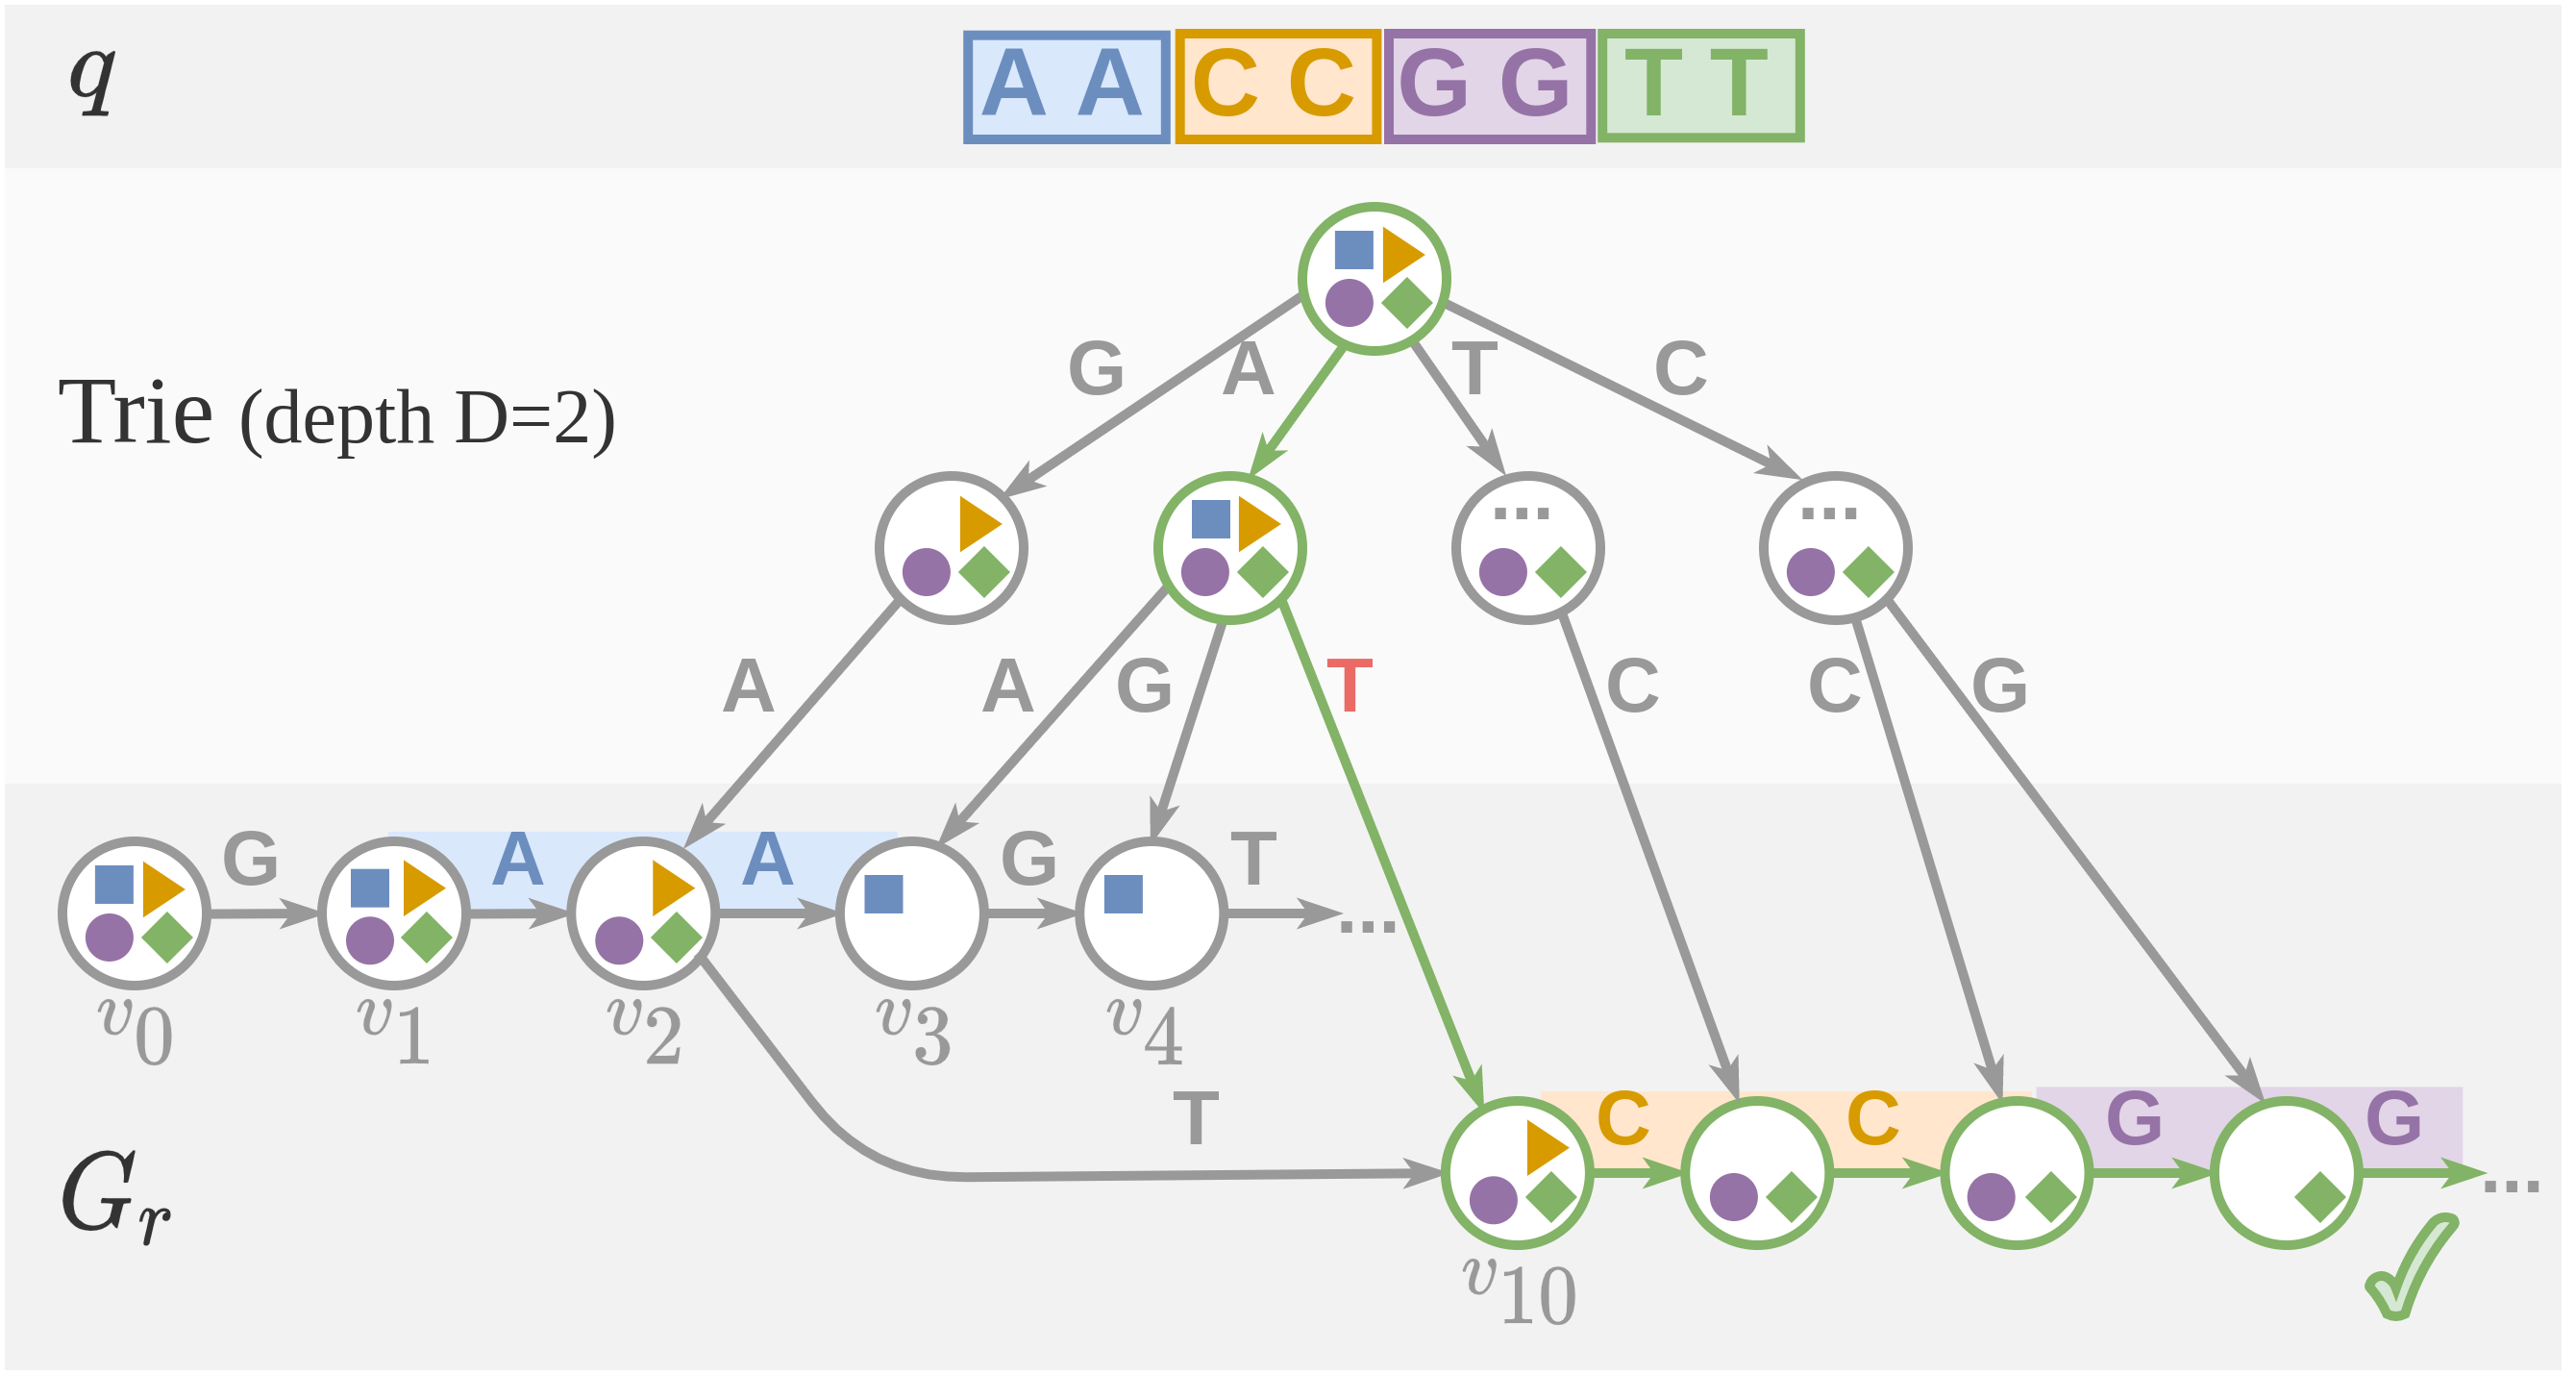
\includegraphics[width=0.6\linewidth]{figures/crumbs-trie.png}
	\caption{Reference graph from \cref{fig:overview}, extended by a trie of
	depth $D=2$. For simplicity, the reverse-complement reference graph and
	parts marked by ``\dots'' are omitted.}
	\label{fig:trie}
\end{figure}

\subsection{Trie index} \label{SEEDsec:trie}
%
Considering all nodes $v \in \RGV$ as possible starting points for the alignment
means that the \A~algorithm would explore all states of the form $\st{v}{0}$,
which immediately induces a high overhead of $\lvert \RGV \rvert$.
%
In line with previous works~\citep{ivanov2020astarix,dox2018efficient}, we avoid
this overhead by complementing the reference graph with a trie index to produce
a new graph $\TG = (\TGV, \TGE)$, where $\TGV$ is the union of the reference
graph nodes $\RGV$ and the new trie vertices, and $\TGE$ is the union of $\RGE$,
the trie edges, and edges connecting the trie leafs with reference nodes. Note
that constructing this trie index is a one-time pre-processing step that can be
reused for multiple queries.

Since we want to also support aligning reverse-complement reads by starting from
the trie \trieroot{}, we build the trie not only from the original reference
graph and also from its reverse-complement.

\para{Intuition}
%
\cref{SEEDfig:trie} extends the reference graph $\RG$ from \cref{SEEDfig:overview} with
a trie. Here, any path in the reference graph uniquely corresponds to a path
starting from the trie \trieroot{} (the top-most node in \cref{SEEDfig:trie}). Thus,
in order to find an optimal alignment, it suffices to consider paths starting
from the trie \trieroot{}, by using state $\st{\trieroot}{0}$ as the only source
for the \A~algorithm.
%
Note that if the reference graph branches frequently, the number of paths with
length $D$ may rise exponentially, leading to an exponential number of trie
leaves. To counteract this exponential growth, we can select $D$ logarithmically
small, as $\log_4N$.

For a more thorough introduction to the trie and its construction,
see~\citep{ivanov2020astarix}. Importantly, our placement of
crumbs~(\cref{SEEDsec:definition}) generalizes directly to reference graphs extended
with a trie (see also \cref{SEEDfig:trie}).

% This leads to the effect that the crumbs in a trie node correspond to the
% union of the crumbs of its descendents (with the exception when crumbs are
% skipped for propagating to the trie \cref{SEEDpara}).

\para{Reusing the trie to find seed matches}
%
As a second usage of the trie, we can also exploit it to efficiently locate all
matches $M(s)$ of a given seed $s$.
%
In order to find all nodes where a seed match begins, we align (without errors)
$\bar{s}$, the reverse-complement of $s$. To this end, we follow all paths
spelling $\bar{s}$ starting from the $\trieroot$---the final nodes of these
paths then correspond to nodes in $M(s)$. We ensure that the seed length $|s|$
is not shorter than the trie depth $D$, so that matching all letters in
$\bar{s}$ ensures that we eventually transition from a trie leaf to the
reference graph.

% Analogously, our computation of crumbs (\cref{SEEDsec:algo} and \cref{SEEDalg:crumbs})
% generalizes directly to reference graphs extended by a trie.
% %
% However, assuming that we select the depth of the trie to be the same as the
% length of each seed ($D=k$) allows us to speed up the computation by only
% starting the search for matches of a seed in~$\varepsilon$.
% %
% Specifically, in \cref{SEEDalg:crumbs}, we can replace \cref{SEEDlin:match-init} by $T
% \gets \{\varepsilon\}$. This is because
% \crefrange{lin:match-forward-start}{lin:match-forward-end} will locate all nodes
% in the original reference graph which can be the end point of a seed match.
% Then, \crefrange{lin:match-backward-start}{lin:match-backward-end} will
% backtrack both in the reference graph as well as in the trie, thus ensuring that
% $M(s)$ is computed correctly.

\para{Optimization: skip crumbs on the trie} \label{SEEDpar:skip_crumbs}
%
Generally, we aim to place as few crumbs as possible, in order to both reduce
precomputation time and avoid misleading the \A~algorithm by unnecessary crumbs.
In the following, we introduce an optimization to avoid placing crumbs on trie
nodes that are ``too close'' to the match of their corresponding seed so they
cannot lead to an optimal alignment.

Specifically, when traversing the reference graph backwards to place crumbs for
a match of seed $s$ starting at node $w$, we may ``climb'' from a reference
graph node $u$ to a trie node $u'$ backwards through an edge that otherwise
leads from the trie to the reference.
%
Assuming $s$ starts at position $i$ in the read, we have already established
that we can only consider nodes $u$ that can reach $w$ with less than
$i+\maxdel$ edges (see \cref{SEEDsec:definition}).
%
Here, we observe that it is sufficient to only climb into the trie from nodes
$u$ that can reach $w$ using more than~$i-\maxins-D$ edges, for
\begin{align}
	\maxins := \left\lceil \frac{\lvert q \rvert \cdot \cmatch + |\seeds| \cdot \delta_{\mli{min}}}{\cins} \right\rceil.
\end{align}
%
We define $\maxins$ analogously to $\maxdel$ to ensure that $\maxins$ insertions
will induce a cost that is always higher than $h\st{u}{i}$. We note that we can
only avoid climbing into the trie if all paths from $u$ to $w$ are too short, in
particular the longest one.

The following \cref{SEEDlem:trie-optimization} shows that this optimization
preserves optimality.

\begin{lem}[Admissibility when skipping crumbs]
	\label{SEEDlem:trie-optimization}
	The \seedh remains admissible when crumbs are skipped in the trie.
\end{lem}
\begin{proof}
	Consider a reference graph with a match of seed $s$ starting in node $w$.
	Now, consider a node $v$ that cannot reach $w$ using more than $i-D-\maxins$
	edges.
	%
	We can then show that a trie node $v'$ with a path to $v$ does not require a
	crumb for the match of $s$ in node $w$.

	Specifically, any path from $\trieroot$ through nodes $v'$ and $v$ to node
	$w$ has total length greater or equal $i-\maxins$. Thus, matching $s$ at $w$
	requires at least $\maxins$ insertions. Hence, the cost of such a path is at
	least $\maxins \cdot \cins = |q| \cdot \cmatch + n \cdot
	\delta_{\mli{min}}$. Observing that this is an upper bound for $h\st{v}{i}$
	concludes the proof.
	%
	\qedwhite
\end{proof}

In order to efficiently identify all nodes $u$ that can reach $w$ by using more
than $i-D-\maxins$ edges (among all nodes at a backward-distance at most
$i+\maxdel$ from $w$), we use topological sorting: considering only nodes at a
backward-distance at most $i+\maxdel$ from $w$, the length of a longest path
from a node $v$ to $w$ is (i)~$\infty$ if $v$ lies on a cycle and
(ii)~computable from nodes closer to $w$ otherwise.

%%\section{Generalizations}
%\todo{Describe mathematically, implement and evaluate}
%
%\subsection{Affine costs}
%
%The state space can be multiplied by the two-element set \{gap opened, gap
%closed\} thus leading to the classical DP problem statement for affine gap costs.
%
%Note that negative costs are not representable because of the triangle
%inequality that both Dijkstra and \A~algorithms rely on for their optimality.
%
%\subsection{Pair reads}
%
%The state space for pair reads is the cross product of the spaces for both
%reads. Every step is made either in the first or the second subspace. The two
%heuristic functions are used (one per read in the pair). in case the two
%substates are too far apart, the cost function is set to $+\infty$, or otherwise
%to the sum of both cost subfunctions. More suffisticated variants of a cost
%function may account more smoothly for the genetic difference between both
%reads.

%\subsection{Phred values}
%
%$$P_{error}(Q) := 10^{-Q/10}$$
%
%We approach the more general task of aligning a read with phred values. To
%account for the phred values, we indivitually modify the costs for matches and
%substitutions depending on the aligned read nucleotide (the cost of insertions
%and deletions does not change). Introducing phred values implies calibrating the
%costs to real probabilities as opposed to abstract relative costs. Thus, we
%distinguish two consequitive tasks: first define the edit costs (by scaling
%the given costs accordingly and applying individual phred corrections), then
%align the read sequence (without phreds) using the modified costs.
%
%\para{Calibrating edit costs}
%\todo{work out the new costs}
%Accounting for phred values in the alignment cost makes matches more expensive
%and substitutions less expensive. This means that even a perfectly matched read will have a cost
%proportional to its length.

%$$\cmatch^\mli{new} \ge \cmatch$$
%$$\csubst^\mli{new} \le \csubst$$

%\para{Aligning with individual edit costs}
%Assume individual edit costs have been already defined to accomodate the
%information from phred values. In order to preserve the \A~correctness, the
%heuristic function must stay optimistic. In case of a matching seed, the exact
%cost for each match and substitution can be computed. For the lack of matching
%seeds, though, an optimistic estimate is
%$$(m-(\mli{maxErrors}+1))*\cmatch + (\mli{maxErrors}+1)*\min(\csubst, \cins,
%\cdel)$$ where $m$ is the read length.

%\subsection{Spliced reads}
%
%Jump edges from every state $\st{u}{i}$ to state $\st{\mli{supersource}}{i}$ can
%stand for an intron and be attributed relatively high costs.

%%%%%%%%%%%%%%%%%%%%%%%%%%%%%%%%%
%\section{Experimental Results}
\section{Evaluation} \label{TRIEsec:eval}
%%%%%%%%%%%%%%%%%%%%%%%%%%%%%%%%%

\begin{samepage}
In this section we present a thorough experimental
evaluation\footnote{\url{https://github.com/eth-sri/astarix/tree/RECOMB2020_experiments}}
of \astarix on simulated Illumina reads. Our evaluation demonstrates that:
\begin{enumerate}
  \item \astarix is faster than \dijkstra because the heuristic reduces the number of explored states by an order of magnitude.
  \item The runtime of \astarix scales better than state-of-the-art optimal
  aligners with increasing graph size, on a variety of reference graphs.
\end{enumerate}
\end{samepage}

\subsection{Implementation \astarix}

Our \astarix implementation uses an adjacency list graph data structure to
represent the reference and the trie in a unified way, representing each letter
by a separate edge object.
%\para{Reverse Complement Alignment}
To represent the reverse complementary walks in $\RG$, the vertices are doubled,
connected in the opposite direction, and labeled with complementary nucleotides
($\texttt{A} \leftrightarrow \texttt{T}$, $\texttt{C} \leftrightarrow
\texttt{G}$).
%
%\para{Default Parameters}
We do not limit the number of memoized heuristic function values
(\cref{TRIEpara:memoization}), but note we could do so by resetting the memoization
table periodically.
%
Our implementation of \dijkstra reuses the same \astarix codebase except the
use of a heuristic function (\ie, with $h \equiv 0$).
\subsection{Setting}
All evaluations were executed singled-threaded on an Intel Core i7-6700 CPU running
at 3.40GHz.

\para{Reference Graphs and Reads}
We designed three experiments utilizing three different reference graphs (in
\cref{TRIEtab:results}). The first is a linear graph without variation based on the
\textit{E.~coli} reference genome (strain: K-12 substr. MG1655,
ASM584v2~\cite{howe2019ensembl}). The other two are variation graphs taken from
the \pasgal evaluations~\cite{jain_accelerating_2019}: they are based on the
Leukocyte Receptor Complex (LRC, with \numprint{1099856} nodes and
\numprint{1144498} edges), and the Major Histocompatibility Complex (MHC1, with
\numprint{5138362} nodes and \numprint{5318019} edges).
%
We note that we do not evaluate on de Brujin graphs, since \pasgal does not
support cyclic graphs.

%\para{Reads}
For the \textit{E.~coli} dataset we used the ART tool~\cite{huang_art_2012} to simulate an
Illumina single-end read set with \numprint{10000} reads of length 100. For the LCR and
MHC1 datasets, we sampled \numprint{20000} single-end reads of length 100 from the already
generated sets in~\cite{jain_accelerating_2019} using the
Mason2~\cite{holtgrewe_mason_2010} simulator.

For \dijkstra and \astarix, the runtime complexity depends not only on the data
size, but also on the data content, including edit costs. More accurate
heuristics lead to better \A performance~\cite{pearl_discovery_1983}, which is
why we evaluate \astarix with costs corresponding more closely to Illumina error
profiles: $\Delta=(0,1,5,5)$.

\para{Metrics}
As all aligners evaluated in this work are provably optimal, we are mostly
interested in their performance.
%
To study the end-to-end performance of the optimal aligners, we use the
Snakemake~\cite{koster_snakemakescalable_2012} pipeline framework to measure the
execution time of every aligner (including the time spent on reading and
indexing the reference graph input and outputting the resulting alignments). We
note that the alignment phase dominates for all tools and experiments.

To judge the potential of heuristic functions, we measure not only the runtime
but also the number of states explored by \astarix and \dijkstra. This number
reflects the quality of the heuristic function rather than the speed of
computation of the heuristic, the implementation and the system parameters.
%"Fig. 3" (it also discusses explored states)}.
%The number of explored states is a more direct indicator for the algorithm's performance
%than the number of expanded states since the algorithm has to generate and consider
%all the neighbors of the states it expands.
%\todo{Harun: this argument only really works
%if computation of the heuristic is not a bottleneck. maybe make that more clear?}
%\subsection{Versions, commands, parameters for running all evaluated approaches}
In the following, we provide details on how we executed the compared tools.

\noindent
\begin{tabular}{lp{9.5cm}}
	\textbf{\pasgal} & \\
	\quad Obtained from & \url{https://github.com/ParBLiSS/PaSGAL} (Commit \texttt{50ad80c}) \\
	\quad Command & \texttt{PaSGAL -q reads.fq -r graph.vg -m vg -o output -t 1} \\
	\textbf{\bitparallel} & \\
	\quad Obtained from &
	\url{https://github.com/maickrau/GraphAligner/tree/WabiExperiments}
	(Commit \texttt{241565c}) \\
	\quad Command & \texttt{Aligner -f reads.fq -g graph.gfa >output} \\
	\textbf{\astarix} & \\
	\quad Obtained from & \astarixurlwithbranch \\
	\quad Command & \texttt{astarix align-optimal -f reads.fq -g graph.gfa >output} \\
	\textbf{\dijkstra} & \\
	\quad Obtained from & \astarixurlwithbranch \\
	\quad Command & \texttt{astarix align-optimal -f reads.fq -g graph.gfa -a dijkstra >output}
\end{tabular}
\subsection{Comparison of Optimal Aligners}

\para{Different Reference Graphs}
\cref{TRIEtab:results} shows the performance of optimal aligners across various
references. On all references, \astarix is consistently faster than \dijkstra,
which is consistently faster than \pasgal and \bitparallel. The memory usage of
\dijkstra is within a factor of 3 compared to \pasgal and \bitparallel. Due to
the heuristic memoization, the memory usage of \astarix can grow several times
compared to \dijkstra.

\begin{table}[H]
\centering
\ra{0.8}
\caption[Performance of optimal aligners for difference references]{Performance
of optimal aligners for different reference graphs.}\label{TRIEtab:results}
\sffamily
%\rowcolors{2}{gray!25}{white}

\renewrobustcmd{\bfseries}{\fontseries{b}\selectfont}
\renewrobustcmd{\boldmath}{}

\begin{tabular}{llrrrr}
\toprule
                && \multicolumn{4}{ c }{\textbf{Runtime} and \textbf{Memory}}\\
                \cmidrule{3-6}
\textbf{Genome graph} & \textbf{Size} & \bfseries \astarix & \dijkstra & \pasgal & \bitparallel\\
\midrule
    \rowcolor{gray!10}
    & &\bfseries \numprint{33} sec	 &\numprint{73} sec &\numprint{3272} sec &\numprint{4906} sec \\
    \rowcolor{gray!10}
    \multirow{-2}{*}{\textit{E. coli} (linear)} & \multirow{-2}{*}{4.7 Mbp} &\numprint{0.66} GB   &\numprint{0.66} GB &\numprint{0.55} GB   &\numprint{0.43} GB \\
    & &\bfseries \numprint{437} sec &\numprint{940} sec	 &\numprint{1614} sec & \\
    \multirow{-2}{*}{LCR (graph)} & \multirow{-2}{*}{1 Mbp} &\numprint{1.12} GB   &\numprint{1.09} GB &\numprint{0.30} GB   & \multirow{-2}{*}{SegFault}\\
    \rowcolor{gray!10}
    & &\bfseries \numprint{1282} sec &\numprint{1588} sec & >\numprint{7200} sec &\\
    \rowcolor{gray!10}
    \multirow{-2}{*}{MHC1 (graph)} & \multirow{-2}{*}{5 Mbp} &\numprint{4.35} GB   &\numprint{1.21} GB    &  \numprint{0.87} GB         		&\multirow{-2}{*}{SegFault}\\
\bottomrule
\end{tabular}

\end{table}

\para{Scaling with Reference Graph Size}
\cref{TRIEfig:scaling_with_graphsize} compares the performance of existing optimal
aligners. \bitparallel and \pasgal always explore all states, thus their
average-case reaches the worst-case complexity of $\Oh(\lvert \AG \rvert) =
\Oh(m \concat \RG)$. Due to the trie indexing, the runtime of \astarix and
\dijkstra scales in the reference size with a polynomial of power around $0.2$
versus the expected linear dependency of \bitparallel and \pasgal.

The heuristic function of \astarix demonstrates a 2-fold speed-up over
\dijkstra. This is possible due to the highly branching trie structure, which
allows skipping the explicit exploration for the majority of starting nodes. 

\begin{figure}[t]
  \begin{subfigure}{.49\textwidth}
    \centering
    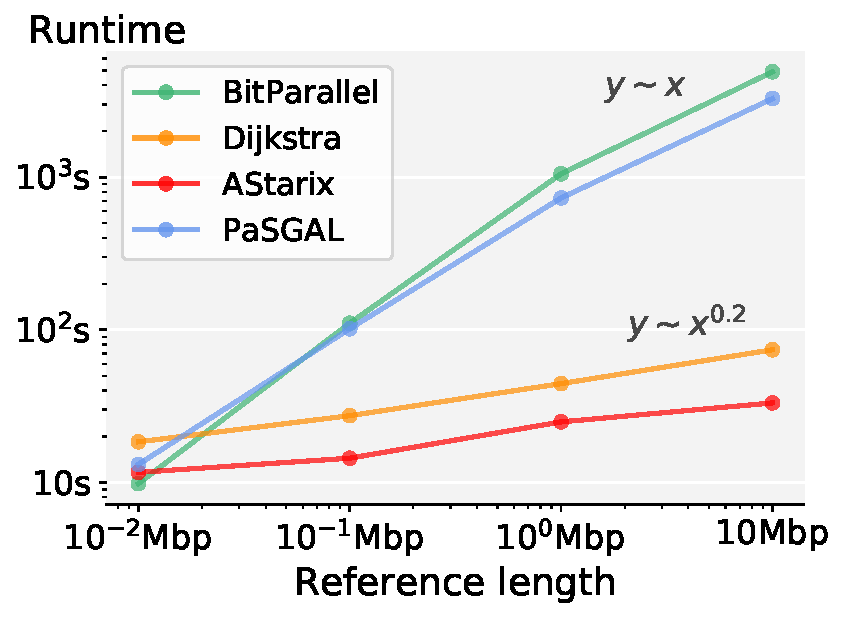
\includegraphics[width=\linewidth]{\dir/figs/cmp/performance_vs_genomesize-head_Mbpxs.pdf}
  \end{subfigure}
  \begin{subfigure}{.49\textwidth}
    \centering
    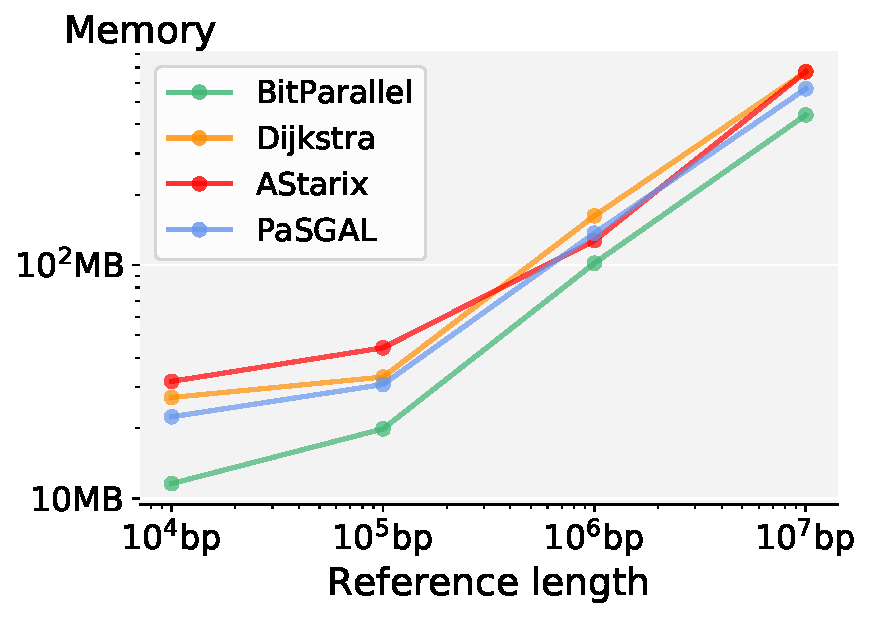
\includegraphics[width=\linewidth]{\dir/figs/cmp/memory_vs_genomesize-headxmax_rss.pdf}
  \end{subfigure}
  \caption{Comparison of overall runtime and memory usage of optimal aligners
     with increasing prefixes of E. coli as references.}
  \label{TRIEfig:scaling_with_graphsize}
\end{figure}

\subsection{\A scaling and speedup}
To measure the speedup caused by the heuristic function, we compare the number
of not only the expanded, but also of explored states (the latter number is
never smaller, see~\cref{TRIEsubsec:general-astar} and the example
in~\cref{TRIEfig:heuristic-benefit}) between \astarix and \dijkstra on the MHC1
dataset.

\cref{TRIEfig:scaling_with_errors} demonstrates the benefit of the heuristic
function in terms of both alignment time and number of explored states. Most
importantly, \astarix scales much better with increasing number of errors in the
read, compared to \dijkstra. More specifically, the number of states explored by
\dijkstra, as a function of alignment cost, grows exponentially with a base of 
around 10, whereas the base for \astarix is around 3 (the empirical complexity is
estimated as a best exponential fit \mbox{$\mli{exploredStates} \sim a \cdot
\mli{score}^b$}).

The horizontal black line in \cref{TRIEfig:scaling_with_errors} denotes the total
number of states $\lvert \RG \rvert \cdot \lvert q \rvert$, which is always
explored by \bitparallel and \pasgal. On the other hand, any aligner must
explore at least $m = \lvert q \rvert$ states, which we show as a horizontal
dashed line. This lower bound is determined by the fact that at least the states
on a best alignment need to be explored.

\begin{figure}[t]
  \begin{subfigure}{.45\textwidth}
    \centering
    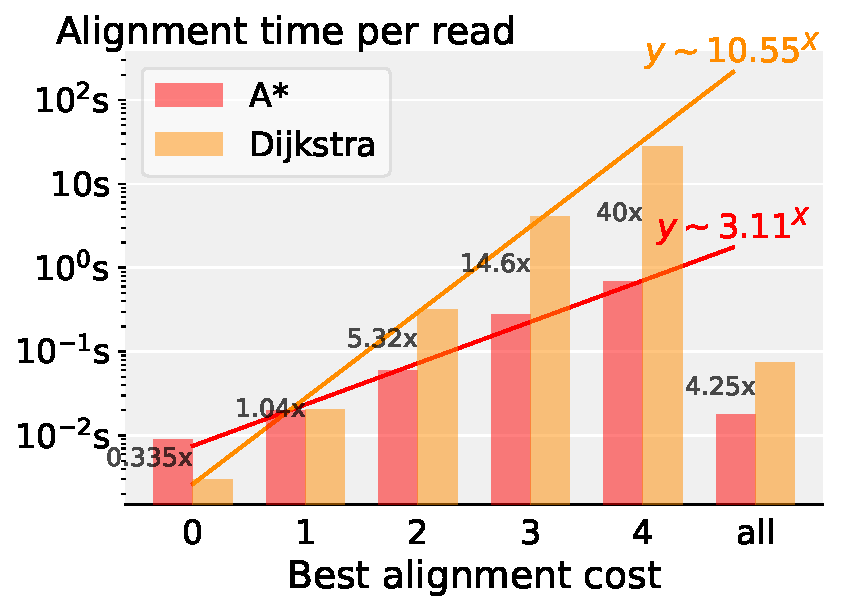
\includegraphics[width=\linewidth]{figs/cmp/heuristic_MHC1_cost-t(map).pdf}
  \end{subfigure}%~\hspace{1em}
  \begin{subfigure}{.45\textwidth}
    \centering
    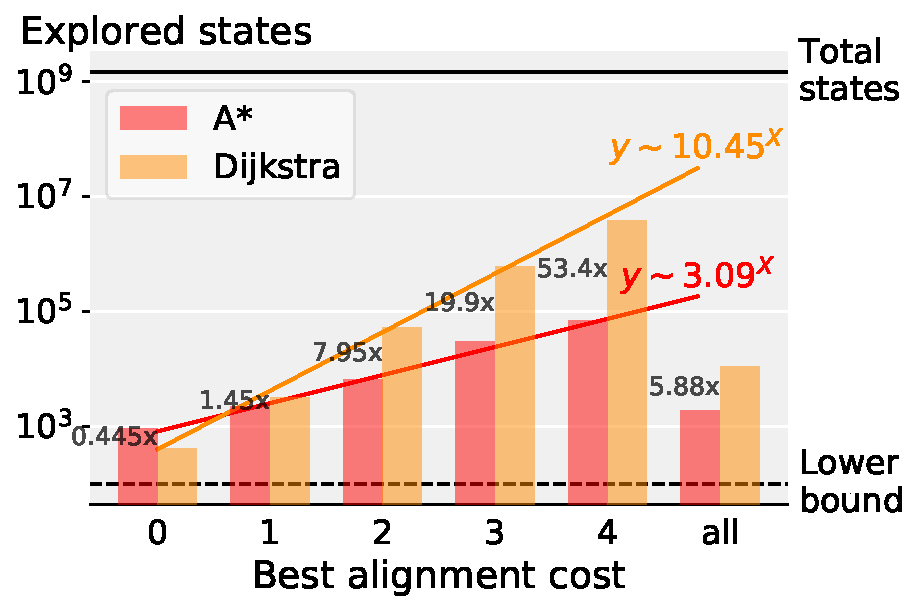
\includegraphics[width=\linewidth]{figs/cmp/heuristic_MHC1_cost-explored_states.pdf}
  \end{subfigure}%
  \caption[Performance scaling with alignment cost]{Comparison of \A and \dijkstra in terms of mean alignment runtime per read and mean explored states depending on the alignment cost on MHC1.}
  \label{TRIEfig:scaling_with_errors}
\end{figure}

\section{Conclusion}
%
We have presented an optimal read aligner based on the \A~algorithm instantiated
with a novel \seedh which guides the search by preferring crumbs on nodes that lead
towards optimal alignments even for long reads.

The memory usage is currently limiting the application of \astarix for bigger
references due to the size of the trie index. A remaining challenge is designing
a heuristic function able to handle not only long but also noisier reads, such
as the uncorrected PacBio reads that may reach 20\% of mistakes. Possible
improvements of the seed heuristic may include inexact matching of seeds,
careful choice of seed positions, and accounting for the seeds order.


% a simple test section that may be deleted
%\input{test-section}

%%%%%%%%%%%%%%
% BODY - END %
%%%%%%%%%%%%%%
% this message marks the end of the body (used to check if we are over the page
% limit)
\message{^^JLASTBODYPAGE \thepage^^J}

%%%%%%%%%%%%%%%%
% BIBLIOGRAPHY %
%%%%%%%%%%%%%%%%
% may be replaced by new bibliography
\clearpage
\bibliography{references}
%\bibliographystyle{genres}  % Genome Research
%\bibliographystyle{rusnat}  % Genome Research
\bibliographystyle{ieeetr}  % RECOMB

%%%%%%%%%%%%%%%%%%%%
% BIBLIOGRAPHY END %
%%%%%%%%%%%%%%%%%%%%
% this message marks the end of the bibliography (used to split the paper from
% the supplement)
\message{^^JLASTREFERENCESPAGE \thepage^^J}

%%%%%%%%%%%%
% APPENDIX %
%%%%%%%%%%%%

% may decide to not include appendix (see "./headers/config/omitappendix.sty")
\ifbool{includeappendix}{%
	\clearpage
	\appendix
	\clearpage
\appendix

\section{Appendix} \label{sec:appendix}
\subsection{Generic Algorithms: \A and \dijkstra} \label{TRIEapp:astar}

\cref{TRIEalg:generic-alignment} shows a generic implementation of the \A algorithm,
roughly following~\cite{dechter_generalized_1985}.
We do not implement the reconstruction of the best alignment in order to simplify the presentation.
The procedure \mbox{\textsc{BacktrackPath}} traces the best alignment back to the $source$, based on remembered edges used to optimize $f$ for each alignment state.
%
\cref{TRIEalg:generic-alignment} also shows a simple implementation of Dijkstra in
terms of \A.

\begin{algorithm}[H]
	\caption{\A algorithm (generalizes Dijkstra)}\label{TRIEalg:generic-alignment}
	\begin{algorithmic}[1]
				
		\Function{\A}{$G\colon \text{Graph}$,
			$S\colon \text{Sources}$,
			$T\colon \text{Targets}$,
			$h\colon \text{Heuristic function}$}
		\State $f \gets \mli{Map}(\mli{default}=\infty)\colon
		\text{Nodes} \to \mathbb{R}_{\geq 0}$
		\Comment Map nodes from $G$ to priorities 
		\State $Q \gets \mli{MinPriorityQueue}(\mli{priority}=f)$ 
		\Comment Priorities according to $f$
		\ForAll{$s \in S$}
			\State $f[s] \gets 0.0$
			\State $Q.\mli{push}(s)$
			\Comment Initially, explore all $s \in S$
		\EndFor
		\While{$Q \neq \emptyset$}
			\State $\mli{curr} \gets Q.\mli{pop}()$
			\Comment Get state with minimal $f$ to be expanded
			\If{$\mli{curr} \in T$}
				\State \Return \Call{BacktrackPath}{$\mli{curr}$}
				\Comment Reconstruct a path to $\mli{curr}$ (omitted)
			\EndIf
				\ForAll{$(\mli{curr},\mli{next},\mli{cost}) \in
				G.\mli{outgoingEdges}(\mli{curr})$}
			\State $\hat{f}_\mli{next} \gets f[\mli{curr}] + \mli{cost} +
			h(\mli{next})$
				\Comment Candidate value for $f[\mli{next}]$
				\If{$\hat{f}_\mli{next} < f[\mli{next}{}]$}
					\State $f[\mli{next}] \gets \hat{f}_\mli{next}$		
					\State $Q.\mli{push}(\mli{next})$
					\Comment Explore state $\mli{next}$
				\EndIf
		\EndFor
		\EndWhile
		\State \textbf{assert} $\mli{False}$
		\Comment Cannot happen if $T$ is reachable from $S$
		\EndFunction

		\Statex

		\Function{Dijkstra}{$G\colon \mli{Graph}$,
			$S\colon \mli{Sources}$,
			$T\colon \mli{Targets}$}
			\State $h(v) \gets 0.0$
			\Comment Constant-zero function $h$
			\State $\Call{\A}{G,S,T,h}$
		\EndFunction
	\end{algorithmic}
\end{algorithm}
           %% HIGHER PRIORITY
\newpage
\subsection{Recursive Alignment Algorithm} \label{app:recursive-align}
\cref{alg:recursiveAlign} shows our implementation of \textsc{RecursiveAlign},
used in \cref{TRIEalg:astarix} to evaluate $h$. \textsc{RecursiveAlign} is a simple
branch-and-bound algorithm that recursively looks for the cheapest alignment of
$s$ starting from $u$, and does not follow paths whose cost exceeds
$\mli{best}$, the best path found so far.

\begin{algorithm}[t]
	\caption{Recursive alignment used by Heuristic in \cref{TRIEalg:astarix}.}\label{alg:recursiveAlign}
	\begin{algorithmic}[1]
		\Statex
			\Function{RecursiveAlign}{$u, s, \mli{curr}, \mli{best}$} \Comment
			Return value is $\leq \mli{best}$
			\If{$\mli{curr} \geq \mli{best}$}
				\State \Return $\mli{best}$
				\Comment Branch and bound: bounding
			\EndIf
			\If{$s = \epsilon$}  % \textbf{or} $u = \mli{border}$}
				\Comment Reached a target
				\State \Return $\mli{curr}$
			\EndIf
			\ForAll{$(u,\mli{v},\ell,w) \in
				\AGE \textbf{ where } \ell \in \{s[0], \epsilon \}$}
				\State $\mli{suff} = s[1:]$ \textbf{if} $\ell \neq \epsilon$ \textbf{else} $s$
				\State $\mli{best} = \Call{RecursiveAlign}{u, \mli{suff}, curr + w, \mli{best}}$
			\EndFor
			\State \Return $\mli{best}$
		\EndFunction
	\end{algorithmic}
\end{algorithm}
       %% HIGHER PRIORITY
%\newpage
\subsection{Parameter Estimation} \label{subsec:parameter_estimation}
We now evaluate the influence of different parameter choices ($\costcap$, $d$,
$D$) on runtime and memory usage.

\begin{figure}[H]
	\centering
	\begin{minipage}{0.48\linewidth}
		\centering
		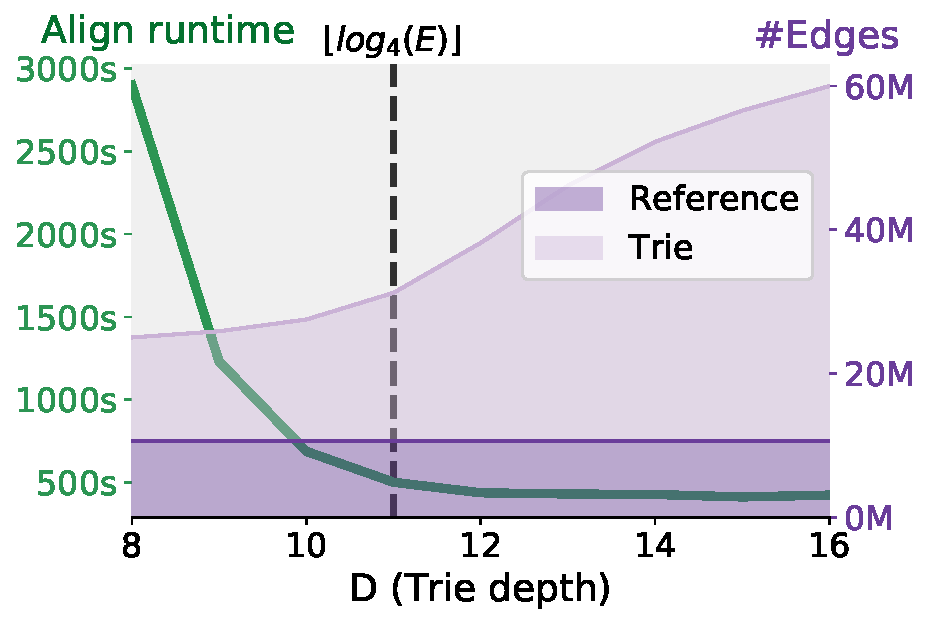
\includegraphics[width=\linewidth]{figs/trie/MHC1-trie-vs-D.pdf}
		\caption[Effect of $D$ on performance of \astarix]{Effect of $D$ on performance of \astarix (MHC1 experiment). The dashed line shows our choice of $D$.}
		%\label{subfig:MHC1-trie_vs_D}
		\label{fig:trie_vs_D}
	\end{minipage}~\hspace{0.7em}
	\begin{minipage}{0.49\linewidth}
		\centering
		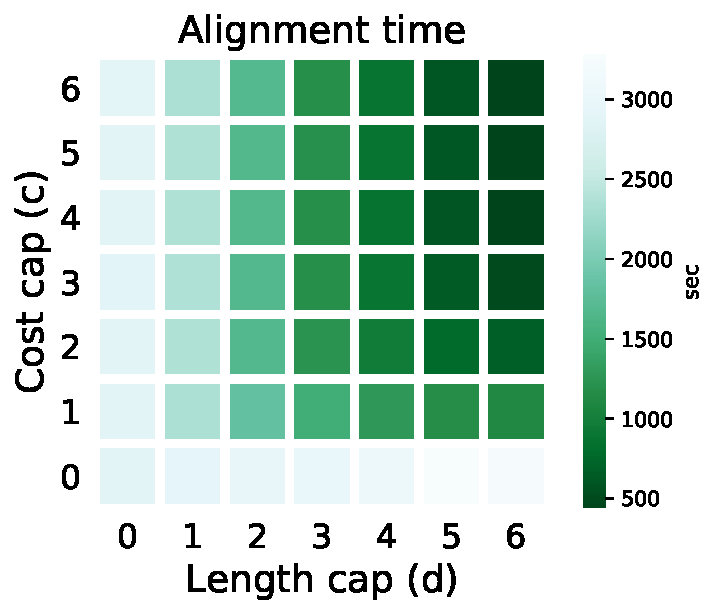
\includegraphics[width=0.8\linewidth]{figs/heuristic/MHC1-heatmap-c_vs_d-align_sec.pdf}
		\caption[Runtime of \astarix depending on $d$ and $\costcap$]{Runtime of \astarix depending on $d$ and $\costcap$ (MHC1 experiment).}
		\label{fig:heuristic-parameters}
	\end{minipage}
\end{figure}

\cref{fig:trie_vs_D} demonstrates the benefit of using a trie with the size
reduction optimization (end of \cref{subsec:trie}): increasing the trie depth
$D$ speeds up aligning but requires more memory. Selecting the trie depth based
on the graph size \mbox{$D = \lfloor \log_\Sigma \lvert \RG \rvert \rfloor$}
provides a reasonable trade-off between alignment time and memory.

\cref{fig:heuristic-parameters} shows the joint effect of $\costcap$ and $d$. It
demonstrates that having a long reach ($d$) that covers at least some errors
($\costcap > 0$) is a reasonable strategy for choosing $d$ and $\costcap$.
%\newpage
\subsection{Versions, commands, parameters for running all evaluated approaches} \label{SEEDsec:commands}
In the following, we provide details on how we executed the newest versions of
the tools discussed in \cref{SEEDsec:eval}:

\para{Executing \astarix} \\
\noindent Obtained from \astarixurl \\
\noindent
\begin{tabular}{lp{9.5cm}}
	\textbf{Seed heuristic} & \\
	\quad Command & \texttt{astarix align-optimal -D 14 -a astar-seeds --seeds\_len l -f reads.fq -g graph.gfa >output} \\
	\textbf{Prefix heuristic} & \\
	\quad Command & \texttt{astarix align-optimal -D 14 -a astar-prefix -d 5 -f reads.fq -g graph.gfa >output} \\
%	\textbf{\dijkstra} & \\
%	\quad Command & \texttt{astarix align-optimal -D 14 -a dijkstra -f reads.fq -g graph.gfa >output}
\end{tabular}

For aligning Illumina reads, \texttt{astarix} is used with additional \texttt{-M
0 -S 1 -G 5} and for HiFi reads with \texttt{-M 0 -S 1 -G 1} which better match
the error rate profiles for these technologies.

\para{Executing other tools} \\
\noindent
\begin{tabular}{lp{9.5cm}}
	\textbf{\vargas} & \\
	\quad Obtained from & \url{https://github.com/langmead-lab/vargas} (v0.2, commit \texttt{b1ad5d9}) \\
	\quad Command & \texttt{vargas align -g graph.gdef -U reads.fq --ete} \\
	\quad Comment & \texttt{--ete} stands for end to end alignment; default is 1 thread \\
	\textbf{\pasgal} & \\
	\quad Obtained from & \url{https://github.com/ParBLiSS/PaSGAL} (commit \texttt{9948629}) \\	
	\quad Command & \texttt{PaSGAL -q reads.fq -r graph.vg -m vg -o output -t 1} \\
	\quad Comment & Compiled with AVX2.\\
	\textbf{\graphaligner} & \\
	\quad Obtained from &
	\url{https://github.com/maickrau/GraphAligner}
	(v1.0.13, commit \texttt{02c8e26}) \\
	\quad Command & \texttt{GraphAligner --seeds-first-full-rows 64 -b 10000 -t 1 -f reads.fq -g graph.gfa -a alignments.gaf >output} (commit \texttt{9948629})\\
	\quad Comment & \texttt{--seeds-first-full-rows} forces the search from all
	possible reference positions instead of using seeds; \texttt{-b 10000} sets
	a high alignment bandwidth; these two parameters are necessary for an
	optimal alignment according to the author and developer of the tool.\\
\end{tabular}\\

\para{Simulating reads}\\
\noindent
\begin{tabular}{lp{9.5cm}}
	\textbf{Illumina} & \\
	\quad & \texttt{art\_illumina -ss MSv3 -sam -i graph.fasta -c N -l 200 -o dir --rnd\_seed 42} \\
	\textbf{HiFi} & \\
	\quad & \texttt{randomreads.sh -Xmx1g build=1 ow=t seed=1 ref=graph.fa illuminanames=t addslash=t pacbio=t pbmin=0.003 pbmax=0.003 paired=f gaussianlength=t minlength=5000 midlength=13000 maxlen=25000 out=reads.fq}\\
	\quad Comment & \texttt{BBMapcoverage}, \url{https://github.com/BioInfoTools/BBMap/blob/master/sh/randomreads.sh} (commit: a9ceda0) \\
\end{tabular}\\        %% LOWEST PRIORITY 
\subsection{Notations} \label{sec:notation}

\cref{tab:notation} summarizes the notational conventions used in this work.

\begin{table}[!h]
	\centering
	\small
	\caption{Notational conventions.}\label{tab:notation}
	\footnotesize \setlength{\tabcolsep}{2.7pt}
	\begin{tabular}{ll}
	\hline
	\textbf{Object}	         & \textbf{Notation}\\
	\hline
	\textbf{Queries}  & $Q = \{ q_i \vert q_i \in \Sigma^m \}$ \\
	\,\, Read            & $q \in Q$ \\
	\,\, Length     & $m := \lvert q \rvert\in \mathbb{N}$\\
	\,\, Position in read & $q[i] \in \Sigma$, $i \in \{0,\dots,m-1\}$\\	
	\hline
	\textbf{Reference graph}& $\RG=(\RGV,\RGE)$\\
	\,\, Size& $\lvert \RG \rvert := \lvert \RGV \rvert + \lvert \RGE \rvert \in \mathbb{N}$\\
	\,\, Nodes& $u, v \in \RGV$\\
	\,\, Number of nodes& $N := \lvert \RGV \rvert \in \mathbb{N}$\\
	\,\, Edges& $e \in \RGE := \RGV \times \RGV \times \Sigma$\\
	\,\, Edge letter& $\ell \in \Sigma$\\
	\textbf{Reference graph with a trie} & $\TG = (\TGV, \TGE)$ \\
	\,\, Trie depth  & $D \in \mathbb{N}_{>0}$\\
	\hline
	\textbf{Alignment graph}& $\AG=(\AGV,\AGE)$\\
	\,\, State& $\langle u,i \rangle \in \AGV := V \times \{0,\dots,m\}$\\
	\,\, Edges& $(\langle u,i \rangle, \langle v,j \rangle,\ell,w) \in \AGE
	\subseteq \AGV \times \AGV \times \Sigma_{\varepsilon} \times
	\mathbb{R}_{\geq 0}$, $\Sigma_{\varepsilon} = \Sigma \cup \{\varepsilon\}$\\
	\,\, Edge cost& $w \in \mathbb{R}_{\geq 0}$\\
	\,\, Alignment& $\pi \in \AGE^*$ and $\sigma(\pi)=q$ \\
	\,\, Alignment cost& $\cost{\pi} \in \mathbb{R}_{\geq 0}$\\
	\hline
	\textbf{Seed heuristic}& $h\st{u}{i}$\\
	\,\, State& $\st{u}{i}$\\
	\,\, Seed length& $k$\\
	\,\, Maximum number of deletions& $\maxdel$\\
	\,\, Maximum number of insertions& $\maxins$\\
	\hline
	\textbf{In all graphs}& $G = (V,E) \in \{ \RG, \AG \}$ \\
	\,\, Walk& $\pi \in G: \pi \in E^*$\\
	\,\, Walk spelling& $\sigma(\pi) \in \Sigma^*$\\
%	\,\, Walk begin and end nodes& $\mli{begin}(\pi), \mli{end}(\pi) \in V$\\
	\,\, Path& A walk without repeating nodes\\
	\hline
	\textbf{\A} & $A^\star(G,S,T,h)$\\
	\,\, Graph& $G=(V,E)$\\
	\,\, Nodes& $u,v \in V$\\
	\,\, Edges& $e \in E \subseteq V \times V \times \Costs$\\ 
	\,\, Source states& $S \subseteq V$\\
	\,\, Target states& $T \subseteq V$\\
	\,\, Heuristic function& $h \colon V \to \Costs$\\
	\,\, Minimum cost to a target& $h^*(u)$\\
	%\,\, Optimistic& $h(u) \leq \min_\pi \cost{\pi}, \pi \colon \pi \text{ starts from } u$\\
	\,\, Explored state & A state pushed to the queue of \cref{alg:astar}\\
	\,\, Expanded state & A state popped from the queue of \cref{alg:astar}\\
	\hline
\end{tabular}
\end{table}        %% LOWER PRIORITY
}{}

\end{document}